\documentclass[a4paper,12.045pt]{ctexart}  

% 加载必要的宏包  
\usepackage{ctex}
\usepackage{geometry} % 用于页面设置  
\usepackage{fancyhdr} % 用于自定义页眉页脚  
\usepackage{longtable}%超级表
\usepackage{tabularray} %线表
\usepackage{appendix} %附录
\usepackage{graphicx}%图片
\usepackage{caption}%编号
\usepackage{amsmath}
\usepackage{listings,matlab-prettifier} % MATLAB 美化包
\usepackage{array} % 用于 m{width} 和 b{width} 类型
\lstset{
	style=Matlab-editor,
	numbers      = left,
	frame        = single,
}

% 页面设置  
\geometry{left=2.5cm, right=2.5cm, top=2.5cm, bottom=2.5cm}  

% 自定义页眉页脚样式  
\pagestyle{fancy}  
\fancyhf{} % 清除默认页眉页脚  
\fancyfoot[C]{\thepage} % 页脚中部显示页码  
\renewcommand{\headrulewidth}{0pt} % 去除页眉横线  
\renewcommand{\footrulewidth}{0pt} % 去除页脚横线  



\ctexset{
	% 修改 section。
	section={   
		name={,、},
		number={\chinese{section}},
		format=\heiti\centering\zihao{4} % 设置 section 标题为黑体、居中对齐、4号字
	},
	% 修改 subsection。
	subsection={   
		format=\heiti\zihao{-4} % 设置 subsection 标题为黑体、小4号字
	},
	subsubsection={   
		format=\heiti\zihao{-4} % 设置 subsection 标题为黑体、小4号字
	}
}

% 设置行间距为默认行距的1.2倍  
\linespread{1.3}  
%\selectfont % 这条命令是必须的，用于使\linespread命令生效 

% 自定义 \maketitle 命令  
\makeatletter  
\renewcommand{\maketitle}{  
	\begin{center}  
		\let \footnote \thanks  
		{\LARGE \@title \par} % 标题  
	\end{center}  
}  
\makeatother  

% 论文题目  
\title{电缆动态载流量预测与周期性规律研究}  
% \date{\today} % 如果不需要日期，可以注释掉这行  
% 自定义摘要标题样式  


% 开始文档  
\begin{document}  
	
	% 显示标题，但不显示页码（如果需要第一页显示页码，请删除 \thispagestyle{empty}）  
	\thispagestyle{fancy} % 如果你想在第一页显示页码  
	%\thispagestyle{empty} % 如果你想在第一页不显示页码  
	\maketitle  
	
	% 摘要和关键词（自定义\keywords命令）  
	\zihao{4}\textbf{\begin{center}	摘要\end{center}}
	\songti\zihao{-4}
	本文旨在深入研究电缆动态载流量的波动情况，通过构建精细模型以预测其变化趋势，并进一步探索其内在的周期性规律。同时，结合电缆动态载流量的实时监测与实际应用，本文深入剖析了弧垂角度、导线温度、环境温度等关键动态增容指标间的相互关联。为了量化分析这些变量间的复杂关系，本文构建了一系列相关模型，旨在揭示它们之间的具体影响机制。
	\par
	在预测电缆动态载流量变化及探究其周期性特征时，本文创新性地将神经网络与时间序列分析相结合，构建了一个高效的预测模型。该模型充分考虑了季节因子和趋势因子对电缆载流量的影响，利用时间序列的季节性分析结果来优化神经网络模型，有效克服了神经网络在预测高波动性数据时可能遇到的挑战。通过整合2019年7月至2020年7月的数据，本文成功预测了2020年8月电缆的载流量，并基于稳态热容平衡方程（涉及导线热功率、日照吸收功率、热辐散热功率和对流散热功率的均衡）对预测结果进行了验证和修正。
	\par
	在探讨环境温度和弧垂角度对电缆载流量的影响时，本文分别构建了基于环境温度和稳态热容平衡方程的关系模型，以及基于弧垂角度与导线温度关系的数学模型。对于环境温度的影响，本文采用了与AA-DLR类似的方法，将环境温度作为自变量，结合稳态热容平衡方程进行分析。而对于弧垂角度与导线温度的关系，本文巧妙地利用斜抛物线形式的悬链线方程进行简化，计算得出悬链线最低点的水平应力，并通过线性回归方法探讨了其与导线温度的关联。进一步地，基于斜抛物线的推导，本文计算了悬垂点应力，并通过多元线性回归分析了其与钢架应力变化的关系。在明确导线温度与弧垂角度的定量关系后，结合导线温度变化与功率的时间积分关系，本文推导出了弧垂角度与导线电流（即钢架应力变化）之间的关联。
	\par
	最后，针对某日用电量激增的情况，本文提出了一套架空输电线路扩容的策略。首先，对现有线路的容量进行评估；其次，预测电流增长的需求；接着，根据实际需求选择合适的增容方式，如增加回路数、优化输电技术等；最后，制定详细的实施计划，确保最大增容量的有效实现。通过这一系列的措施，本文为解决输电线路增容问题提供了实用的指导方案。
	\par \quad
	\par \quad
	\par \quad

	\par\noindent
	\heiti 关键词：
	\songti\zihao{-4}神经网络；时间序列；稳态热容平衡方程；斜抛物线；最低点水平应力
	\pagebreak
	% 正文开始  
	\section{问题重述}  
	\subsection{问题背景}
	在电力系统中，架空输电线路（OHTL）作为电力传输的核心，其输电效率直接关系到国民经济的稳定与发展。然而，随着电力需求的不断增长，输电线路面临的环境挑战也愈发严峻。特别是在高峰时段，导线过热、弧垂降低等安全隐患成为制约输电效率和线路安全的关键因素。为解决这些问题，动态增容技术（DLR）应运而生。其中环境调节式DLR（AA-DLR）只考虑环境温度的变化，而不考虑其他影响，因环境温度对导线温度的影响有限，导线温度变化很小，几乎看成是不变的。而实时监测式DLR（RTM-DLR）通过实时收集导线温度、弧垂角度等关键数据，为输电线路提供精确的容量调整依据。因此，利用RTM-DLR技术深入研究输电线路的动态载流量需求，并分析环境因素对其影响，对于提升电力系统的安全性和稳定性具有极其重要的意义。
	
	\subsection{问题内容}
	本研究以架空输电线路动态增容系统为研究对象，基于在线监测装置（Overhead Temperature Line Monitoring, OTLM）收集的实时数据，建立数学模型，以解决以下关键问题：
	\par
	1.动态载流量预测：选取OTLM1设备的采样数据，建立数学模型，预测2020年8月的动态载流量需求，并分析以下不同时间间隔（30分钟、1小时、2小时、4小时、8小时、16小时、32小时、64小时）的载流量变化情况，并探究电流的周期性特征。
	\par   
	2.温度与弧垂对载流量的影响：综合考虑OTLM1和OTLM2的采样数据，探讨温度、弧垂角度对载流量的定量影响。
	\par 
	3.导线电流与钢架应力关系：针对具有L型切面的四脚钢结构架空输电线路，建立数学模型，分析导线电流变化与钢架腿部每侧应力变化之间的关系。
	\par
	4.增容方案与最大增容量确定：假设2020年8月15日用电量有大幅度增加，请提出一套可行的增容方案，并计算出该方案下的最大增容量。
	\section{问题分析} 
	\subsection{问题一的分析}
	问题一的核心在于预测2020年8月的架空输电线路动态载流量需求，并深入分析其电流的周期特征。要达成此目标，关键在于理解什么是动态载流量以及得到架空输电线路载流量随时间变化的规律。
	\par
	首先，我们需要明确架空输电线路载流量的定义。载流量，即在特定条件下，导体能够持续承载而不导致其稳定温度超过预设限值的最大电流值，与即时导线电流大小无关。多种因素如导线温度、环境温度、风速、导线材质、太阳辐射以及截面积等都会影响架空输电线路的载流量。为简化模型及数据处理，我们将主要关注导线温度、环境温度、太阳辐射、导线材质和截面积的影响。
	\par
	通过问题背景得知，传统的载流量值受一组固定的保守天气假设的限制，称之为静态热额定值（STR）。研究表明，实际线路额定值在大多数情况下高于STR，故研究人员提出了动态热额定值（DTR）系统。DTR即动态载流量，它与OTLM收集的导线实时状态挂钩，可以充分利用线路客观存在的隐性容量，提高载流量，比保守的STR更具有实用性。此时，导线载流量满足稳态热平衡方程[2]。
	\par
	根据稳态热平衡方程，当导线和外界温度的热交换达到稳定时，电流将保持稳定。该值即为该架空输电线路在该状态下的载流量。对于导线材质和截面积，我们将依据国标进行查询确定。
	\par
	基于题目附件提供的OTML1和OTML2检测的从2019年7月至2020年7月的导线温度与环境温度数据，我们将进行细致的数据预处理和分析。通过拟合两者的时间曲线，我们能够更准确地把握其变化趋势。
	\par
	在数据分析阶段，我们将运用时间序列分析和神经网络模拟等方法进行频谱分析，以识别出温度数据中的主要周期性成分。这些周期性成分可能对应于一天内的不同时间段（如白天和夜晚）或一周内的不同天数（如工作日和周末）。通过预测2020年8月的导线温度与环境温度数据，并结合稳态热平衡方程，我们可以进一步预测出具有周期特征的8月份载流量数据。
	\subsection{问题二的分析}
	在问题二的分析中，我们需综合考虑OTLM1和OTLM2的采样数据，以深入剖析温度与弧垂角度对载流量的具体且定量的影响。我们将特别关注环境温度、导线温度以及弧垂角度这三个核心因素，并探究它们如何共同作用于载流量。
	\par
  	首先，鉴于AA-DLR模型在仅考虑环境温度作为单一因素对载流量影响时存在的局限性，我们决定从稳态热平衡方程的角度出发，将环境温度作为自变量，深入探索其与载流量之间的确切关系。这种方法有助于我们更全面地理解环境温度如何直接和间接地影响载流量的变化。
	\par
	其次，导线温度作为影响载流量的另一重要参数，其与电阻率之间的直接联系决定了载流量的波动。为了精确分析导线温度对载流量的影响，我们将设定环境温度为常量，并利用稳态热平衡方程推导出导线温度与载流量之间的定量关系。这将为我们提供一个清晰的视角，以了解导线温度对载流量变化的贡献。
	\par
	最后，我们不能忽视弧垂角度对载流量的潜在影响。导线在不同温度下的长度变化会导致弧垂角度的相应调整，而由于档距和电线塔高度固定，这种变化将直接影响弧垂的大小。为了具体分析这种影响，我们将运用悬链线方程来确定弧垂角度与悬链线最低点水平应力之间的关系，进而发现悬链线最低点水平应力与导线温度之间的显著线性关系。基于这些分析，我们将能够推导出弧垂角度与导线温度之间的定量关系，并进一步推导出弧垂角度与载流量之间的定量关系。这将使我们能够更全面地理解这些因素对载流量的综合影响。
	\subsection{问题三的分析}
	问题三要求我们全面分析导线电流变化与钢架腿部每侧应力变化之间的内在关联。在此，我们将以弧垂角度为关键桥梁，通过两个不同角度的推导，来揭示它们之间的定量关系。
	\par
	首先，从悬链线方程出发，我们可以将其简化为斜抛物线方程，进而计算得到斜抛物线水平最低点的应力值。基于先前问题的线性回归结果，我们能够确定水平应力与导线温度之间的定量关系。随后，通过计算瞬时功率对时间的积分，我们能够得到热量的变化，并进一步将其转化为导线温度。这样一来，我们就成功地将弧垂角度与电流之间的关系进行了定量表达。
	\par
	其次，利用斜抛物线公式，我们可以计算出两条悬链线端点对于悬挂点的力。考虑到弧垂角度的影响，我们进行矢量合成，得到一个合力。然后，我们利用这个合力值对四条钢架腿部的数据进行多元线性回归分析，从而得出钢架腿部每侧应力变化与弧垂角度之间的定量关系。
	\par
	由此，我们利用弧垂角度作为连接点，成功地将钢架腿部应力变化与电流变化之间的关系进行了定量分析。
	\subsection{问题四的分析}
	问题四要求我们提出一套增容方案并确定最大增容量。为达成此目标，我们将遵循以下五个步骤：
	\par
	1.评估现有线路容量：首先，我们需要对现有的输电线路容量，即载流量进行全面评估，以准确了解当前线路的负载能力。这一评估将基于问题一中已预测的载流量数据，确保我们对线路当前状态有清晰的认识。
	\par
	2.确定增容需求：接下来，我们将根据2020年8月15日预计的用电量增加情况，计算出需要增加的线路容量。这一计算将基于附件中提供的2019年7月至2020年8月每日所用电流数据，通过深入的数据分析，我们能够预测出未来的用电增长趋势，从而确定增容的具体需求。
	\par
	3.选择增容方式：在确定增容需求后，我们将选择适合的增容方式。这可能包括提升导线截面、增加回路数、优化输电技术等多种方案。我们将综合考虑技术可行性、经济成本、施工难度等因素，选择最适合当前线路和用电需求的增容方式。
	\par
	4.制定实施计划：选定增容方式后，我们将制定详细的实施计划。这包括施工时间、材料采购、人员安排等方面的具体规划。我们将确保计划合理、可行，并能够在规定的时间内完成增容工作，以满足用电需求。
	\par
	5.确定最大增容量：最后，在综合考虑技术限制、经济限制、现有线路的负载能力、杆塔结构的承载能力、地形条件、环境因素等多方面因素后，我们将确定一个合理的最大增容量。这一增容量将确保线路在增容后能够稳定运行，同时满足未来的用电需求。
	
	
	\section{模型假设} 
	1.为简化数据处理与运算，我们假设架空输电线路为光亮新线符合并遵循国标，采用35/8的钢芯铝绞线电阻作为其主要导体材料[5]。
	\par   
	2.为便于数据处理，我们假设架空输电线的悬链线模型可以近似为斜抛物线模型[6]，这一假设在大多数情况下能够提供良好的近似效果。
	\par   
	3.由于我们是以天为单位研究架空输电线路的性质，因此假设每一天内的载流量保持不变，忽略一天内可能出现的细微变化。
	\par
	4.在以天为单位的研究中，我们假设日平均温度能够代表这一天中每时每刻的温度，这一假设在大多数情况下是合理的。
	\par
	5.同样地，在以天为单位计算每天导线平均的日照辐射强度时，我们假设正午太阳高度角能够代表这一天中每时每刻的太阳高度角，从而简化计算过程。
	\par
	6.为简化计算过程，假设该架空输电线路所用材料钢芯铝绞线中的电阻率与纯铝的电阻率相当。这一假设基于铝作为钢芯铝绞线主要导电材料的事实。
	\par
	7.为防止产生歧义，统一假设本题中架空输电线路（OHTL）所在地纬度采取北纬，经度采取东经。
	\section{符号说明} 
	对本文在描述中用到的所有的符号加以阐释和说明。
	\begin{center}
		\begin{longtable}{>{\centering\arraybackslash}m{5cm}>{\centering\arraybackslash}m{9cm}} 
			
			\caption*{表一} \\
			\hline \multicolumn{1}{c}{\textbf{符号}} & \multicolumn{1}{c}{\textbf{说明}} \\ \hline 
			\endfirsthead
			
			\multicolumn{2}{c}%
			{{\bfseries \tablename\ \thetable{} -- 续表}} \\
			\hline \multicolumn{1}{c}{\textbf{符号}} & \multicolumn{1}{c}{\textbf{说明}}\\ \hline 
			\endhead
			
			\hline \multicolumn{2}{l}{{下页续}} \\ 
			\endfoot
			
			\hline
			\endlastfoot
			$I$  & 导线电流强度 \\
			$R$  & 交流电阻 \\
			$R_{d}$  & 直流电阻 \\
			$t_{c}$  & 导线温度 \\
			$t_{a}$  & 环境温度 \\
			$T_{0}$  & 导线初始温度 \\
			$v$  & 导线附近风速 \\
			$Q_{s}$  & 日照吸收功率 \\
			$Q_{c}$  & 对流散热功率 \\
			$Q_{r}$  & 辐射散热功率 \\
			$D$  & 导线直径 \\
			$\operatorname{Re}$  & 雷诺数 \\
			$\varepsilon$  & 导体表面辐射系数 \\
			$\sigma$  & 斯蒂芬-玻尔兹曼度常数 \\
			$\alpha$  & 导线表面吸热系数 \\
			$q_{s}$  & 导线所处地日照辐射强度 \\
			$\alpha _{sol}$  & 太阳高度角 \\
			$\omega$  & 到现所在地纬度 \\
			$\delta$  & 太阳直射点纬度 \\
			$k$  & 集肤效应系数 \\
			$QL$  & 下四分位数 \\
			$QU$  & 上四分位数 \\
			$IQR$  & 四分位间距$QU-QL$ \\
			$\lambda_{f}$  & 导线表面空气膜热传导率 \\
			$\theta $  & 弧垂角度 \\
			$h $  & 电塔高度差 \\
			$l $  & 档距，电塔水平距离\\
			$\beta $  & 其正切值为电塔高度差与档距之比\\
			$\sigma_{0} $  & 悬链线最低点处水平应力大小\\
			$f $  & 弧垂\\
			$C $ & 比热容\\
			$k $ & 线性回归比例系数\\
		\end{longtable}
	\end{center}

	
	
	\section{模型的建立与求解}
	\subsection{问题一的模型建立与求解}
	\subsubsection{数据预处理}
	在建立模型之前，我们首先对题目附件中提供的为期一年的以时间为自变量的数据进行了细致的处理，这些数据涵盖了Line Temperature等共计70项指标。具体处理步骤如下：
	\par
	1.指标筛选：针对问题要求，我们直接剔除了包括Stress1 Ch1 Fcross在内的8项指标，这些指标在全数据集中均为0，对建模没有实际价值。
	\par
	2.异常值处理：对剩余的62项指标，我们采用了箱线图四分位检测法来识别并剔除异常值。具体而言，所有落在$QL-1.5IQR$以下或$QU+1.5IQR$以上的值均被视为异常值并予以剔除。同时，为了保持数据的完整性，我们对剔除异常值的位置进行了线性插值处理。如图一所示，我们选取了其中四项指标的箱型图作为示例，图中箱外的点均已被剔除。
	\begin{figure}[h]
		\small
		\centering
		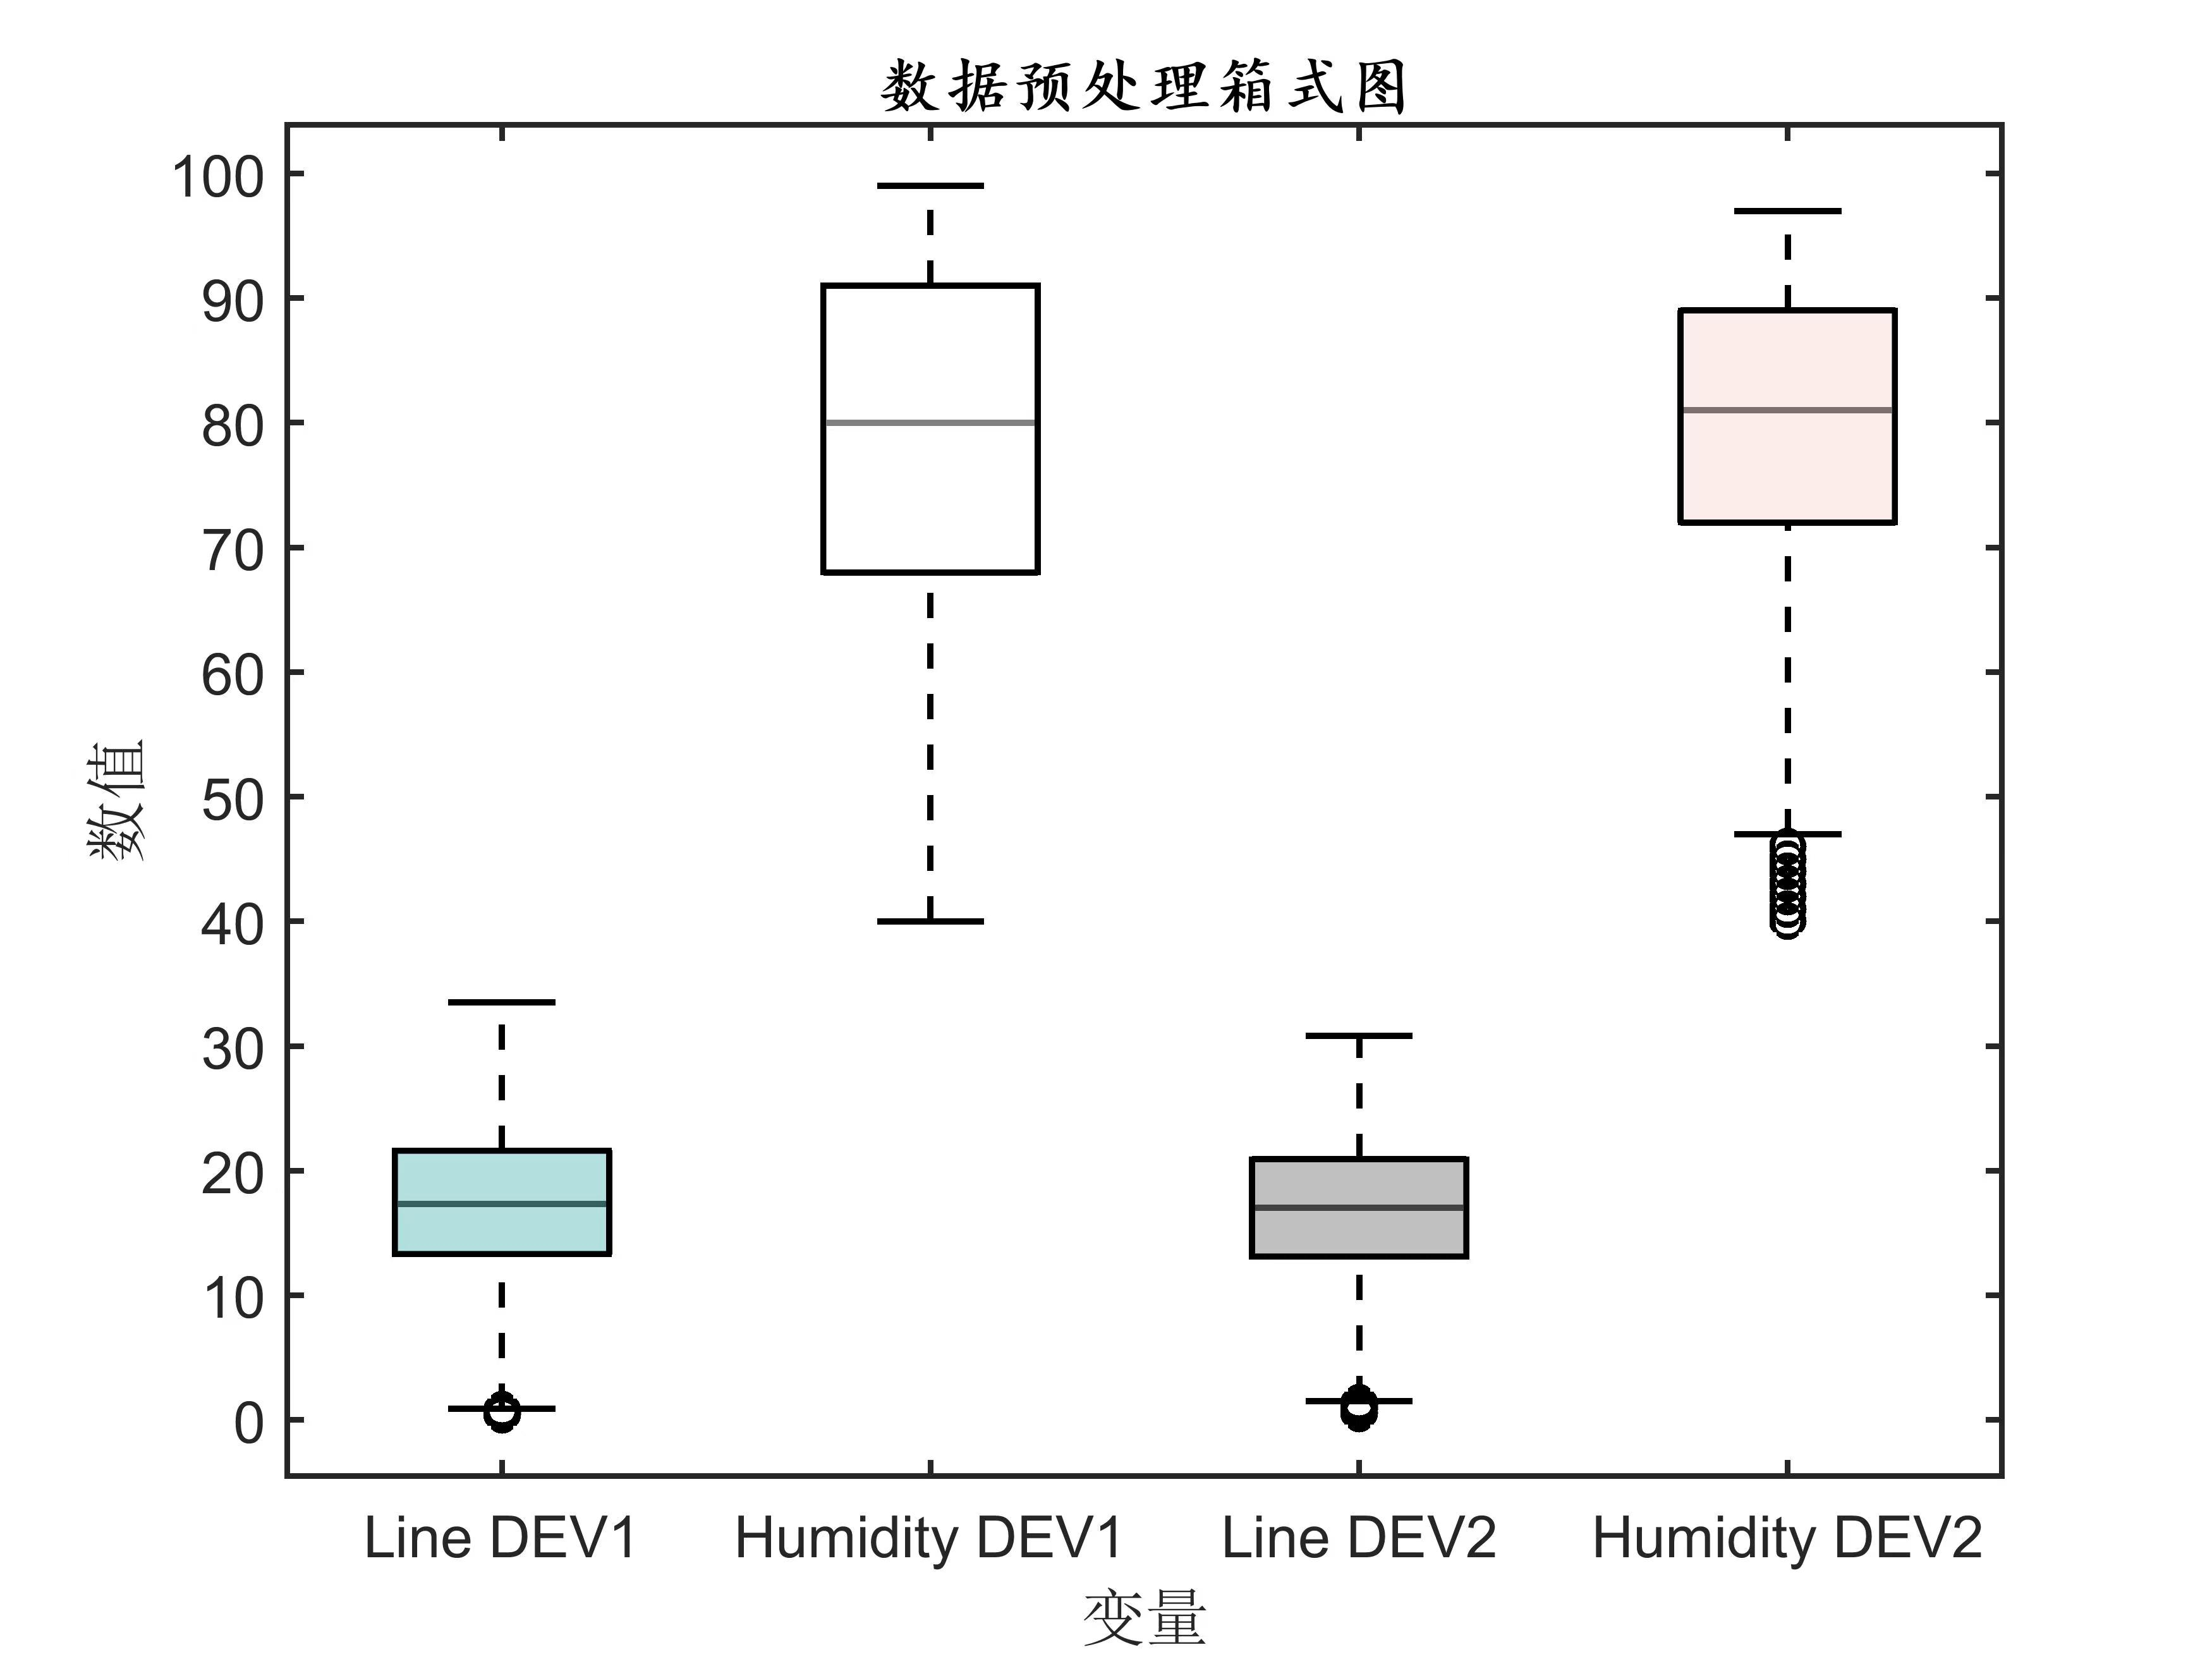
\includegraphics[width=11cm]{figure/箱线图.jpg}
		\caption*{图一}
	\end{figure}
	\par
	3.等距时间间隔调整：由于附件中提供的Date/Time数据并非等距分布，为了确保后续数据处理与分析的便利性，我们对部分样本进行了添加与删除的调整。经过这一步骤，所有数据的Date/Time变量均按照10分钟的间隔呈现等距分布。
	\par
	4.缺省值处理：对于在调整Date/Time样本过程中产生的新缺省值，我们同样采用了MATLAB中的三次样条插值的方法进行处理，以确保数据的连续性和完整性。
	\par
	经过以上步骤的处理，我们得到了最终预处理完的数据集。
	\subsubsection{模型建立}
	本模型的建立过程分为两大关键部分：温度预测与稳态热平衡方程的应用。
	\par
	1.神经网络与时间序列预测的结合
	\begin{figure}[h]
		\small
		\centering
		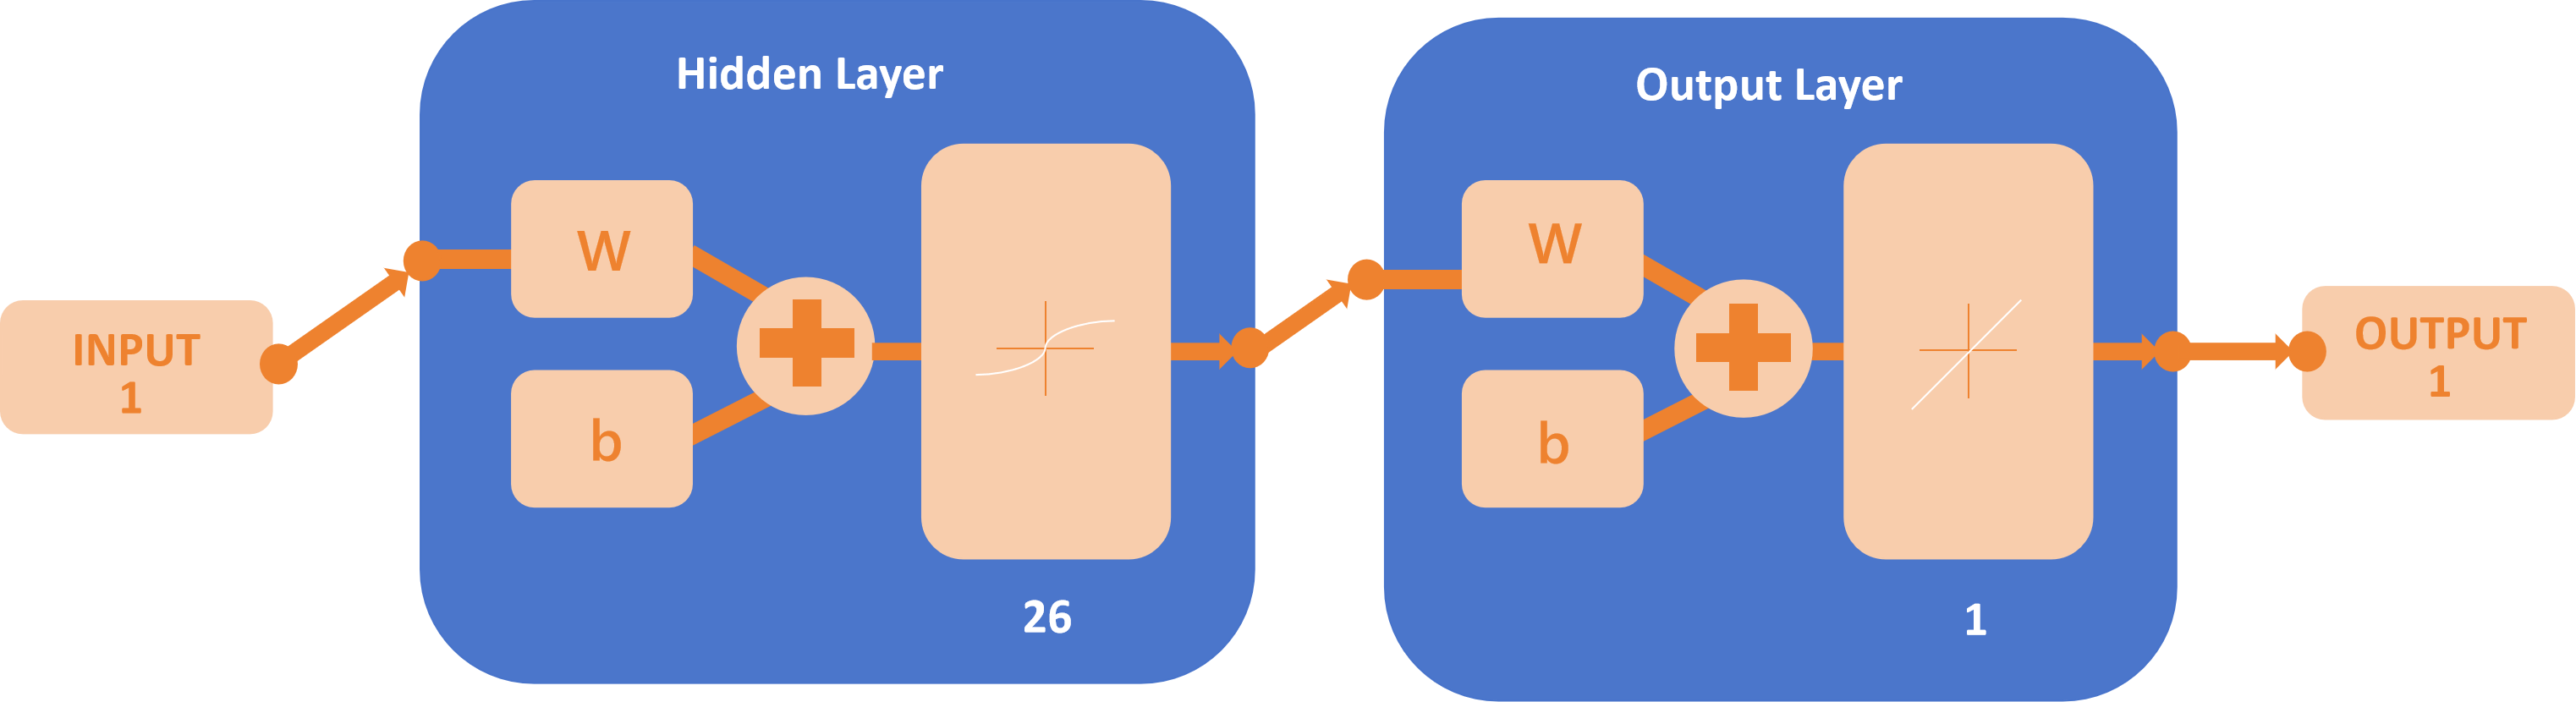
\includegraphics[width=13cm]{figure/神经网络预测.png}
		\caption*{图二}
	\end{figure}
	\par
	在温度预测阶段，我们发现单独使用神经网络或时间序列分析进行拟合时，效果均不理想。因此，我们创新性地将两者相结合，拟合效果得到了显著提高。具体实施步骤如下：
	\par
	1)我们首先整合了附件中2019年7月至2020年7月期间的数据，对每一天的导线温度和环境温度进行均值处理，得到了一套完整的每日温度均值数据集。然后通过神经网络进行训练，从而预测出2020年8月份每天的平均导线温度和环境温度。
	\begin{figure}[h]
		\small
		\centering
		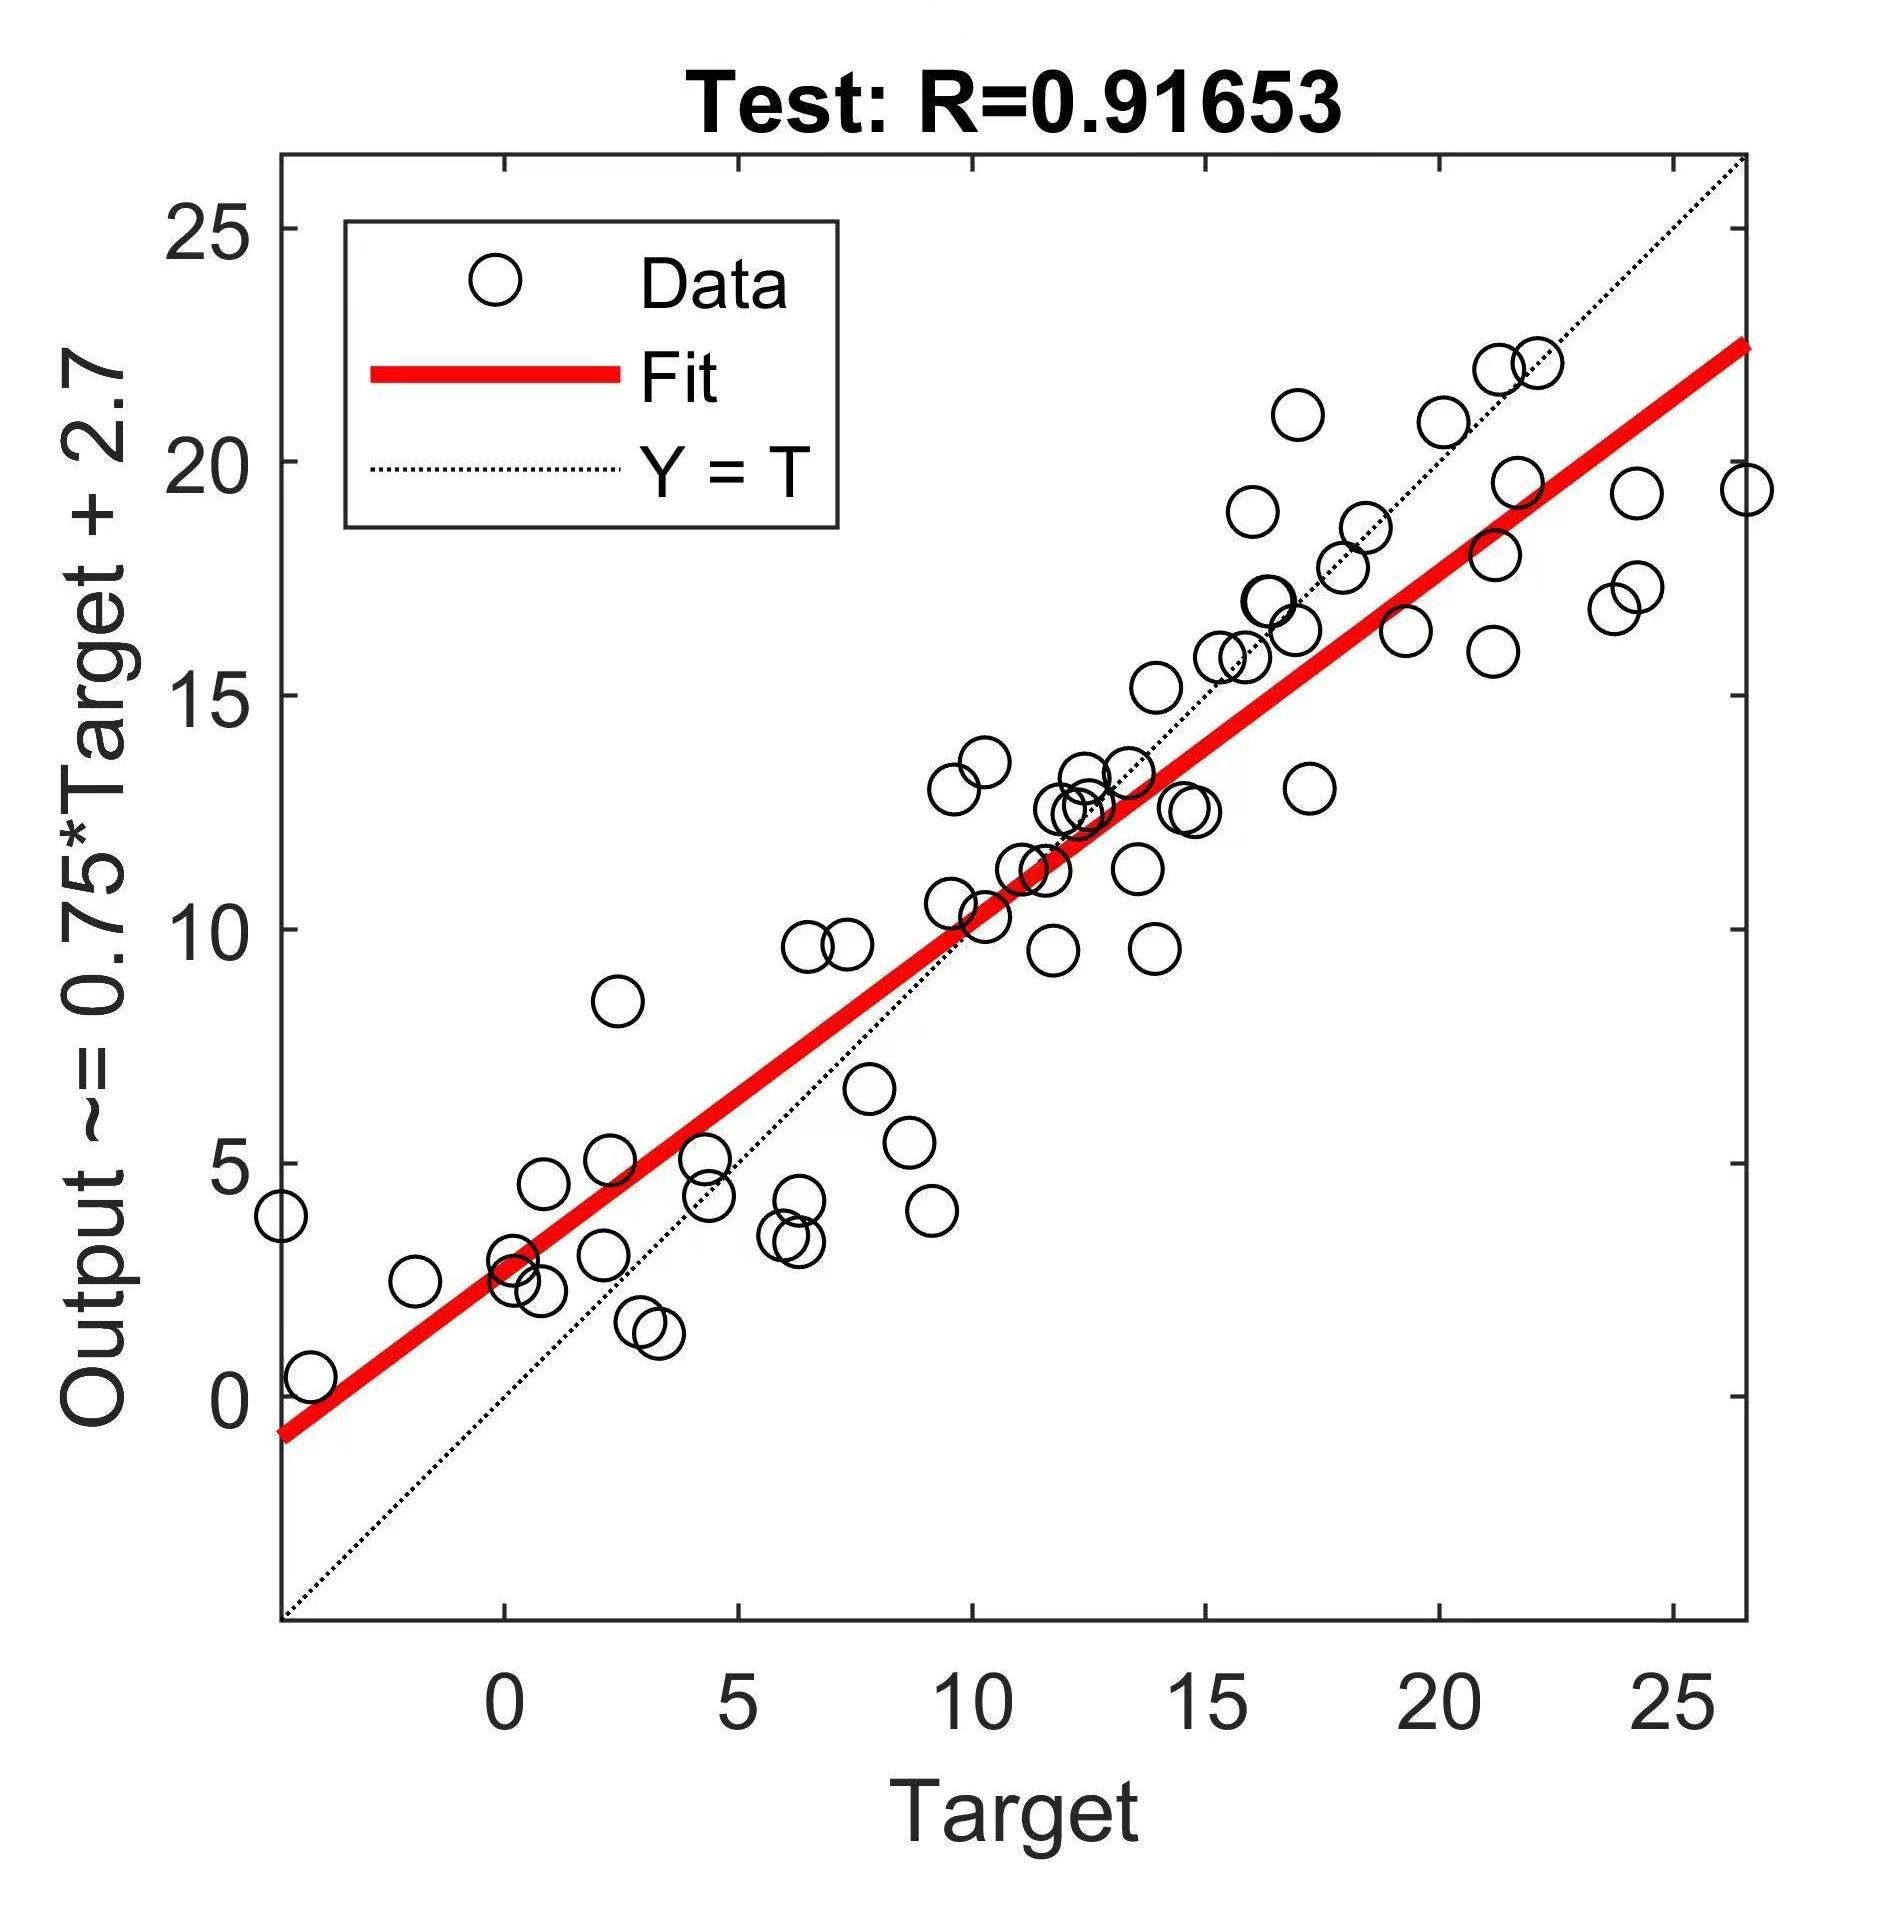
\includegraphics[width=8cm]{figure/神经网络拟合优度.jpg}
		\caption*{图三}
	\end{figure}
		\par
	图三说明神经网络拟合的优度很好，训练集、测试集、验证集的拟合优度都很高。
	\par
	图四与图五将部分原始数据曲线与拟合预测出的曲线进行对比，展现出拟合优度很高，可以用来进行2020年8月份每天的平均导线温度和环境温度的预测。
	\begin{figure}[htbp]
		\centering
		\begin{minipage}[t]{0.48\textwidth}
			\centering
			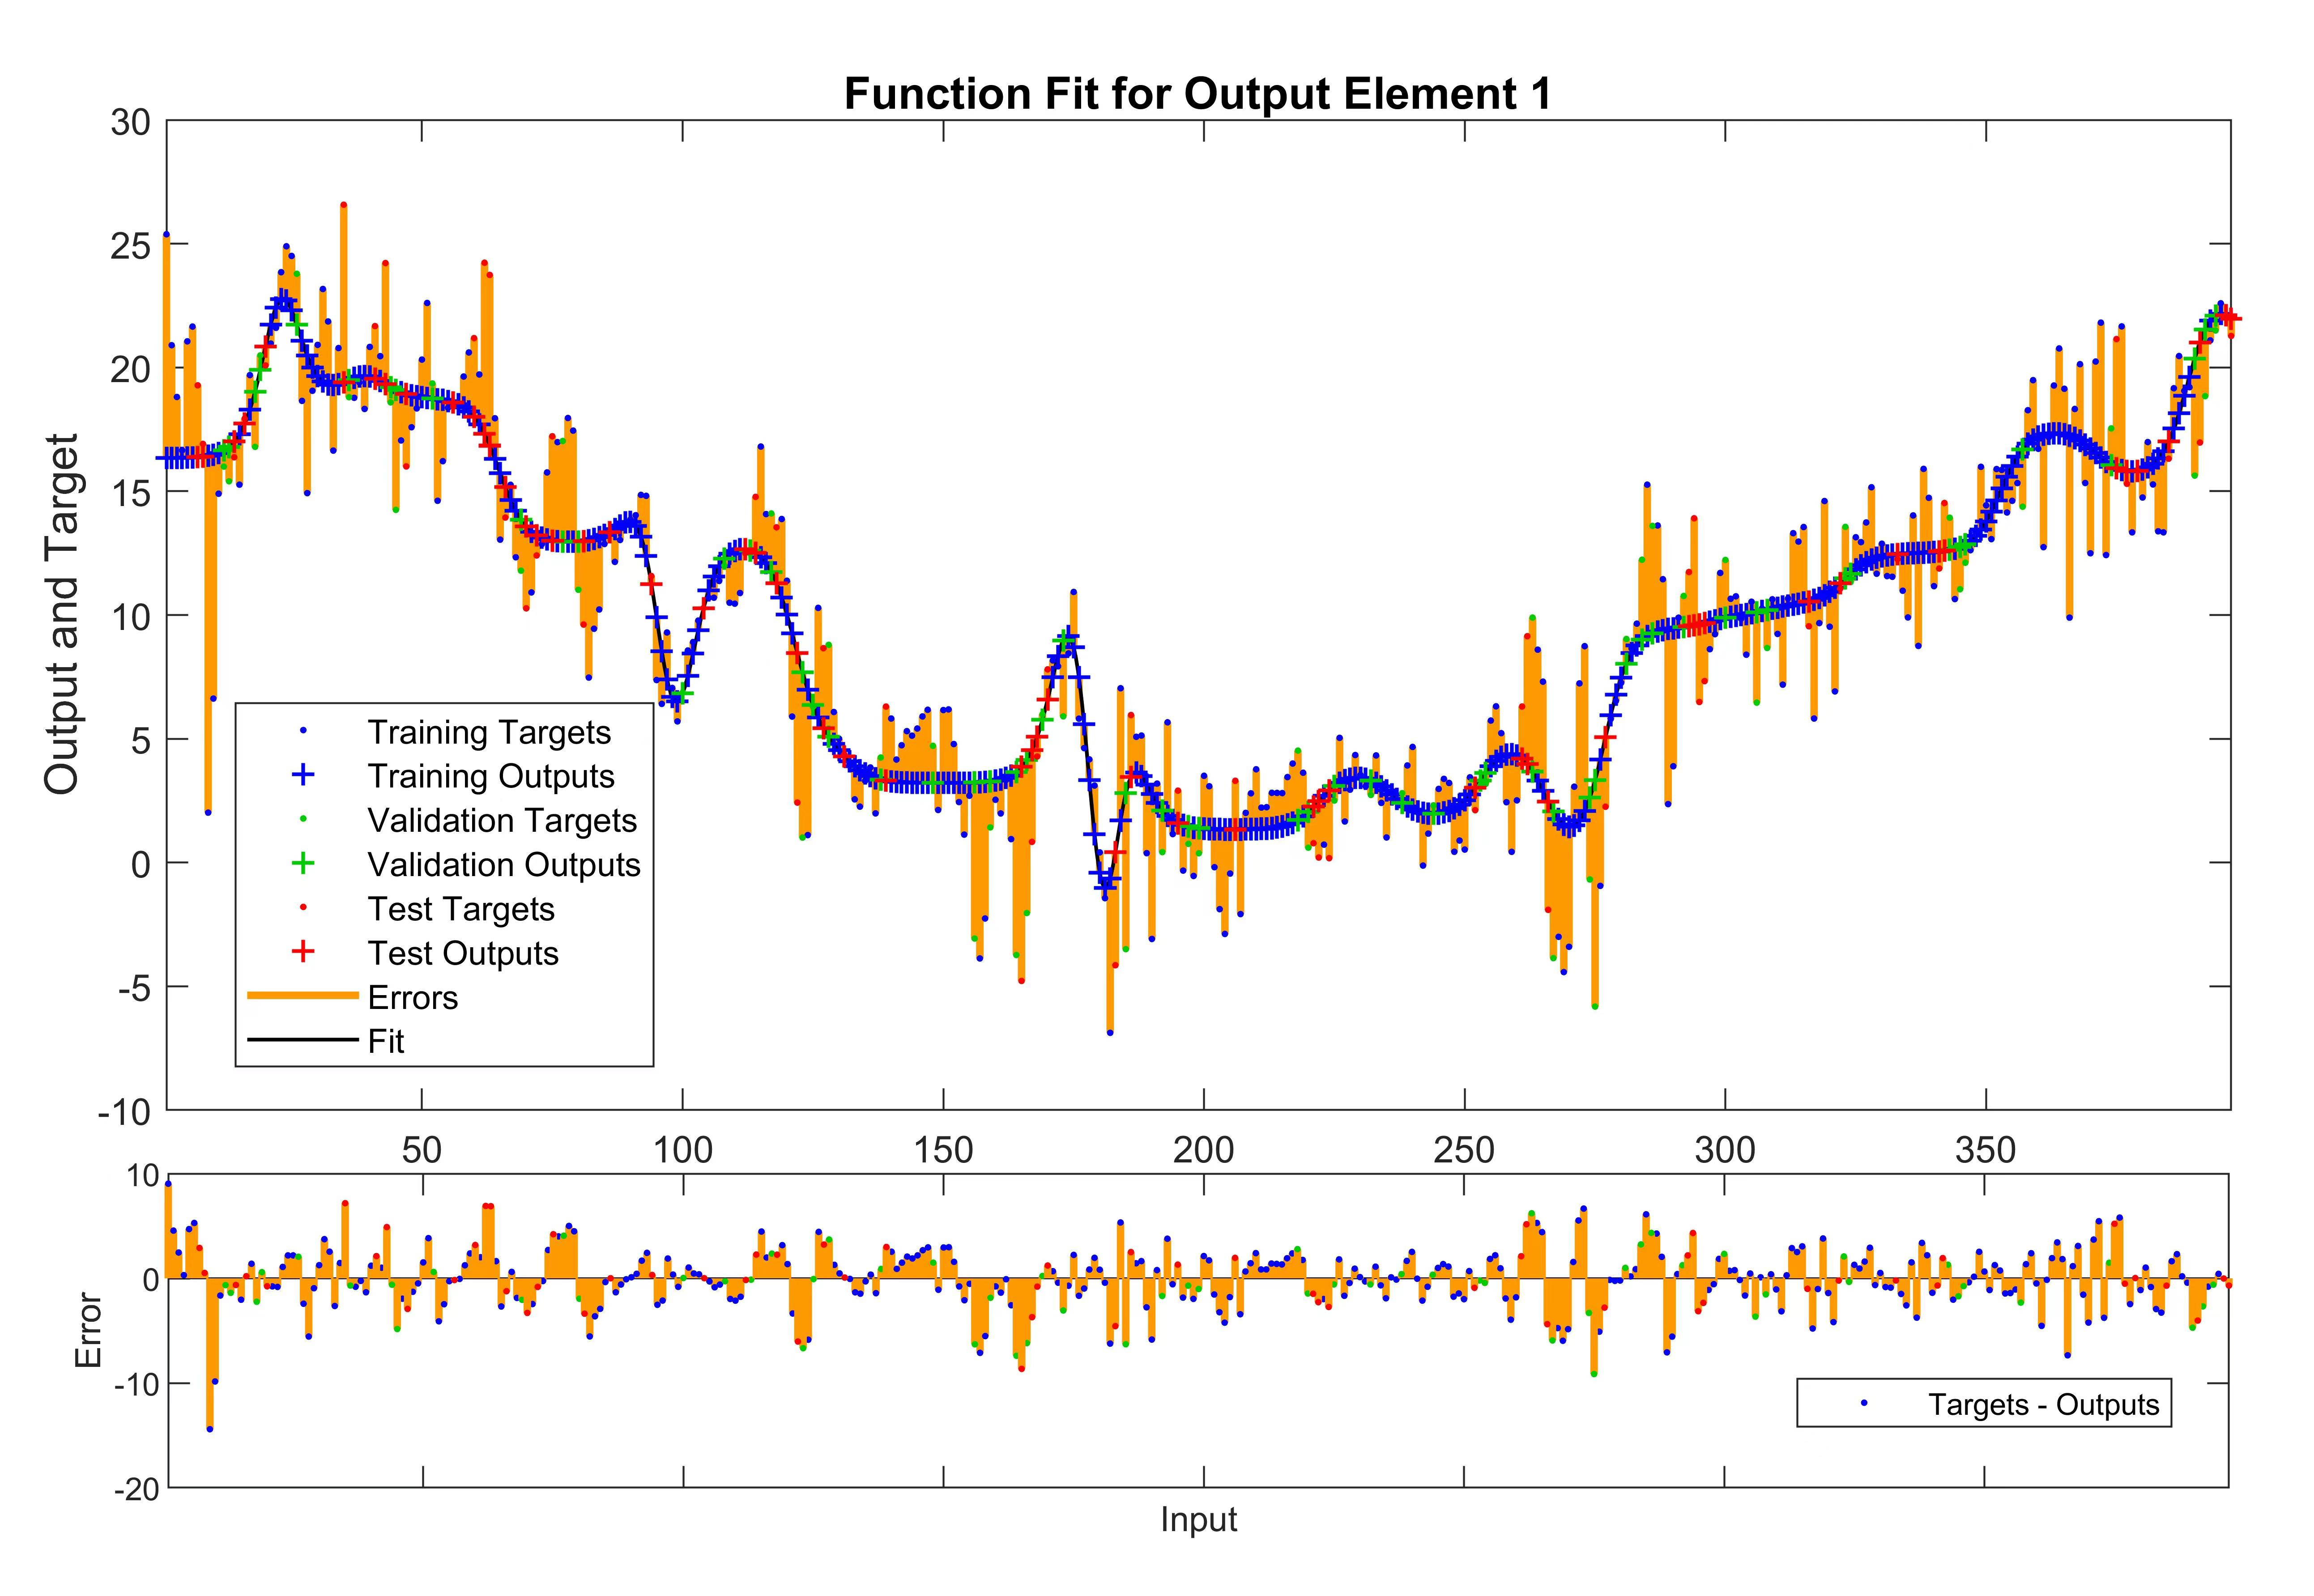
\includegraphics[width=9cm]{figure/神经网络拟合.jpg}
			\caption*{图四}
		\end{minipage}
		\begin{minipage}[t]{0.48\textwidth}
			\centering
			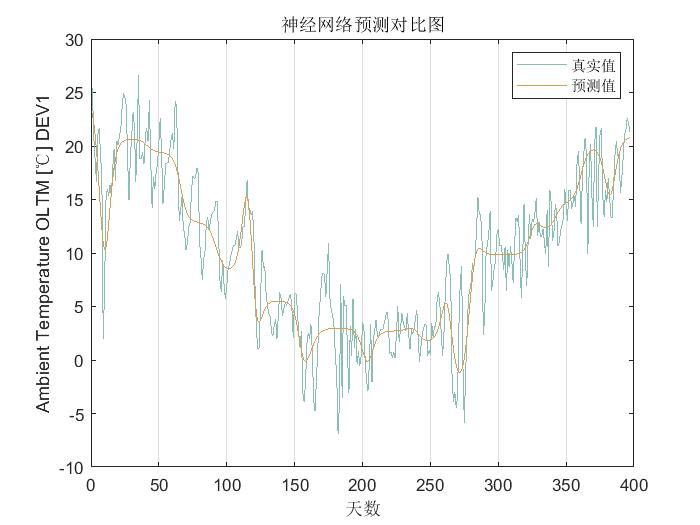
\includegraphics[width=8cm]{figure/神经网络拟合2.jpg}
			\caption*{图五}
		\end{minipage}
	\end{figure}

	\par
	2)随后，我们运用时间序列分析技术，以24小时为周期对温度数据进行季节性分解，从而提取出每小时对应的季节因子(具体数值见附录)。
	\begin{figure}[h]
		\small
		\centering
		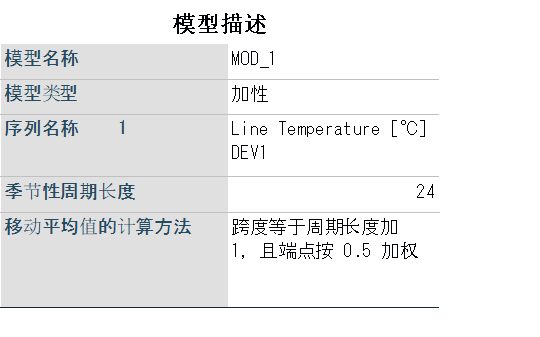
\includegraphics[width=12cm]{figure/季节因子介绍.png}
		\caption*{}
	\end{figure}
	\par
	3)最后，我们将神经网络预测出的每日导线温度均值和环境温度均值与通过时间序列分析获得的季节因子相结合，成功预测出2020年8月份每天每小时的导线温度均值和环境温度均值。
	\par
	2.稳态热平衡方程[2]的使用
	\begin{equation}
		I^2 R\left(t_{c}\right)+Q_{s}=Q_{c}+Q_{r}
	\end{equation}
	\par
	方程(1)左边热功率与日照吸收功率$Q_{s}$促使导线温度升高，右边对流散热功率$Q_{c}$与辐射散热功率$Q_{r}$促使导线温度降低，方程等式成立时，电线电流与温度状态达到稳态平衡。
	\par
	1) 求取对流散热功率
	\par
	顾名思义，对流散热是空气流体与导线表面接触时产生的热传递。
	\begin{equation}
		Q_{c}= 0.57\lambda _{f}\times \operatorname{Re}  ^{0.71} \times \pi (t_{c} -t_{a} )
	\end{equation}	
	\par
	通过公式(2)可以得到$Q_{c}$，其中参数 $\lambda _{f}$和$ \operatorname{Re}$分别由(3)和(4)确定。
	\begin{equation}
		\lambda _{f} =2.42\times 10^{-2} +7\times 10^{-5}\left[t_{a}+\frac{1}{2}\left(t_{c}-t_{a}\right )\right ] 
	\end{equation}
	\par
	根据《电力工程电气设计手册》[1]中公式(4)可以确定参数$\operatorname{Re}$的大小。
	\begin{equation}
		\operatorname{Re}=1.644 \times 10^9 v D\left[t_{\mathrm{a}}+0.5\left(t_{\mathrm{c}}-t_{\mathrm{a}}\right)\right]^{-1.78}
	\end{equation}
	\par
	$\operatorname{Re}$为雷诺数，是一个用来反映气流行为的无量纲参数。由公式四可以确定此时导线附近空气流体的$\operatorname{Re}$值。其中$v$代表风速，对于架空输电线路这种大跨度类型的设施，一般令其为0.6m/s。而导线直径$D$采取9.60mm这一标准[5]。
	\par
	2)求取辐射散热功率
	\par
	导线不断以热辐射的形式向温度比它低的外界放出热量，那么就有对应的辐射散热功率。其大小由公式(5)确定。
	\begin{equation}
		Q_{r}=\pi \varepsilon D \sigma\left[\left(t_{\mathrm{c}}+273\right)^4-\left(t_{a}+273\right)^4\right]
	\end{equation}
	\par
	参数$\varepsilon$为导线表面的辐射系数，该参数在导线为光亮新线时取值在0.23-0.46之间，此处取均值0.345。参数$\sigma$为斯蒂芬-玻尔兹曼常数，值取$5.67×10^{-8}\left ( m^{2} \cdot K^{4}  \right ) $。
	\par
	3)求取日照吸收功率
	\par
	导线会吸收部分太阳辐射功率，使其升温，具体日照吸收功率由公式(6)[3]可以得到。
	\begin{equation}
		Q_{s}=\alpha D q_{s}
	\end{equation}
	\par
	参数$\alpha$ 为导线表面的吸热系数，有$\alpha==\varepsilon$。参数$q_{s}$为导线所处环境日照辐射强度，可以由Haurwitz经验公式，即公式(7)得到。
	\begin{equation}
		q_{s}=1098\cos (\alpha _{sol} )e^{\frac{-0.057}{\cos (\alpha _{sol} )} } 
	\end{equation}
	\par
	其中参数$\alpha _{sol}$为太阳高度角，根据理想化假设，一天中的太阳高度角都取为正午太阳高度角。则该角度可由公式(8)得到。
	\begin{equation}
		\alpha _{sol}=90^{\circ} -\left | \omega\pm \delta  \right | 
	\end{equation}
	\par
	其中当地纬度在题目附件中已经给出，为避免误差维度最终求均值确定。而直射点纬度$\omega$随日期产生变化，可以根据公式(9)确定,其中$n$代表当年的第$n$天。
	\begin{equation}
		\omega=23.45^{\circ}\times\sin(\frac{2\pi\left ( 284+n \right )  }{365} )
	\end{equation}	
	\par
	4)求取导线交流电阻$R$
	\par
	对于tc下的交流电阻R来说，应当考虑到集肤效应影响，得到其实际电阻。
	\begin{equation}
		R\left (  t_{c} \right ) =\left ( 1+k \right ) R_{d} 
	\end{equation}
	\par
	公式十一展示了$t_{c}$下，其交流电阻与直流电阻的关系，其中参数$k$为集肤效应系数，查询《电力工程电气设计手册》，由于导线横截面积小于400$m^{2}$，$k$取0.0025。同时对于任何温度($t_{c}$)的直流电阻$	R_{dc}$与20°下的直流电阻都满足公式(11)。
	\begin{equation}
		R_{dc}=R_{20}\left[1+\alpha_{20}\left(t_{c}-20\right)\right]
	\end{equation}
	\par
	已知公式中20℃时导线材料的温度系数$\alpha_{20}$为0.00403,同时用此温度下铝的直流电阻代替以钢芯铝绞线为原材料的导线电阻，约为$2.65\times10^{-8}\Omega$ 。
	\par
	5)得出每日的载流量
	\par
	通过公式(1)到公式(11)，最终可以计算出每一天的导线载流量。将通过神经网络和时间序列预测得到的2020年8月份的每天的环境温度与导线温度代入上述11个公式，便可以预测到8月每一天的载流量数据。
		\begin{figure}[h]
		\small
		\centering
		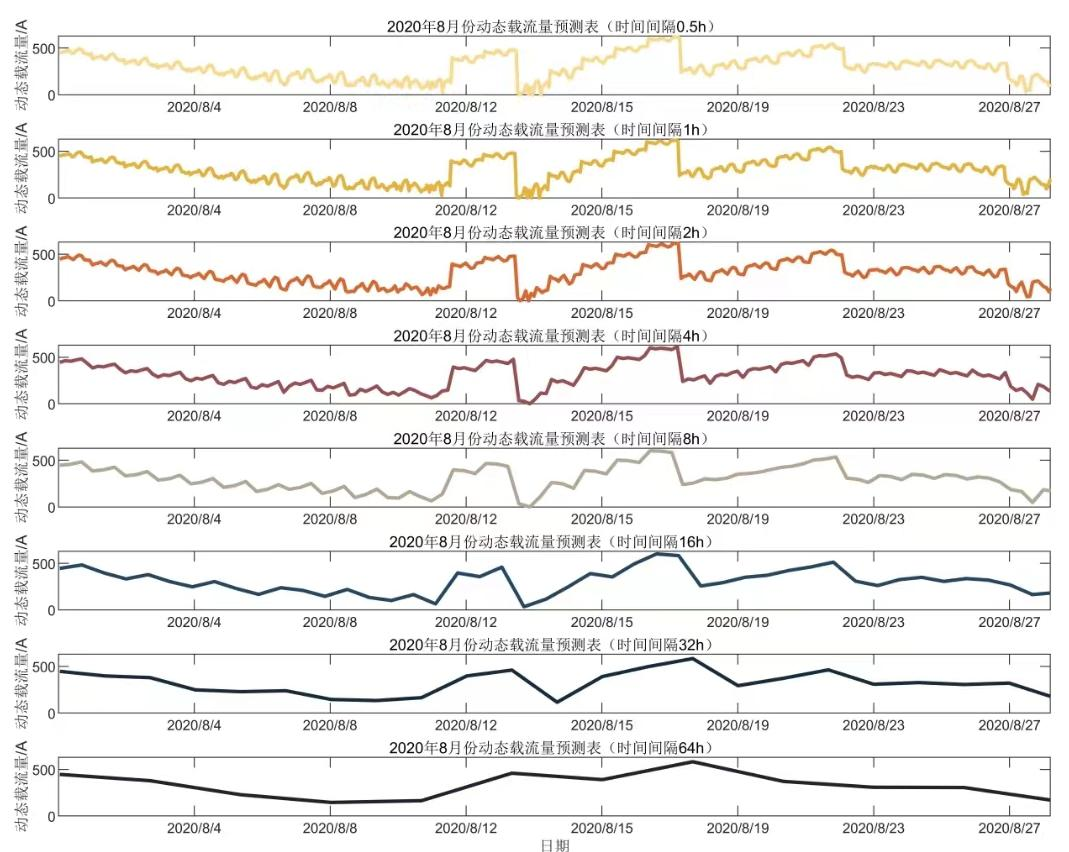
\includegraphics[width=13.5cm]{figure/预测表.jpg}
		\caption*{图六}
	\end{figure}
	\subsubsection{模型求解与结果分析} 
		通过神经网络和时间序列预测以及稳态热平衡方程的使用，最终得到了图六。
	从时间间隔较小的预测图中很明显能看出具有一定的以天为一个周期的周期性质，因为昼夜交替，温度变化等，使得他们呈现锯齿状，并不是单调的。但是当时间间隔拉长，比如32h,64h，此时图中基本展示不出周期性质，而是接近于平缓状态。
	
	\subsection{问题二的模型建立与求解}
	本体建立模型主要从三个角度考量：环境温度、导线温度和弧垂角度对载流量的影响。其中，两种温度分别对于载流量的影响可以通过公式(1)稳态热平衡方程变形得到。故该题主要在于弧垂角度对载流量的定量影响需要建模求解。由于弧垂角度与载流量的直接关系不好寻找，故我们先建模寻找导线温度与弧垂角度的定量关系，然后关联导线温度对载流量的影响，得到结论。
	\subsubsection{数据获取}
	\begin{figure}[h]
		\small
		\centering
		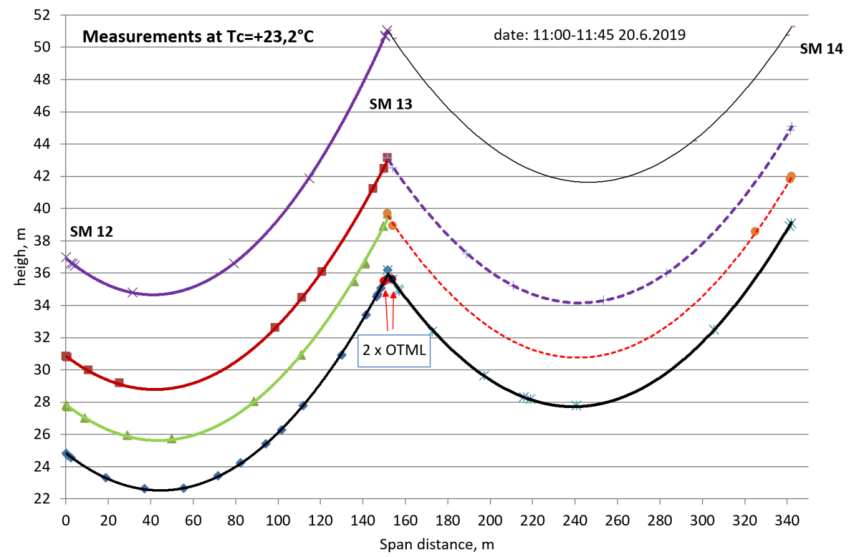
\includegraphics[width=16cm]{figure/OTML位置示意图.png}
		\caption*{图七}
	\end{figure}
	\par
	观察图七(题目附图)，可以确定塔SM12与SM13的档距大约在$160m$，高度差大约在$14m$，而SM13与SM14的档距大约在$180m$，高度差大约在$2m$。同时从问题附表中可以获知，两个OTML设备获得的导线温度以及悬垂角度的大量实时数据。该数据在第一个问题中已经进行过预处理。
	\subsubsection{模型建立}
	问题中是三个塔，两条导线，我们将原题一般化，其实就是两个悬链线系统。故我们选择直接研究悬链线模型，得到普遍结论。图八是我们做的简易悬链线示意图。
	\begin{figure}[h]
		\small
		\centering
		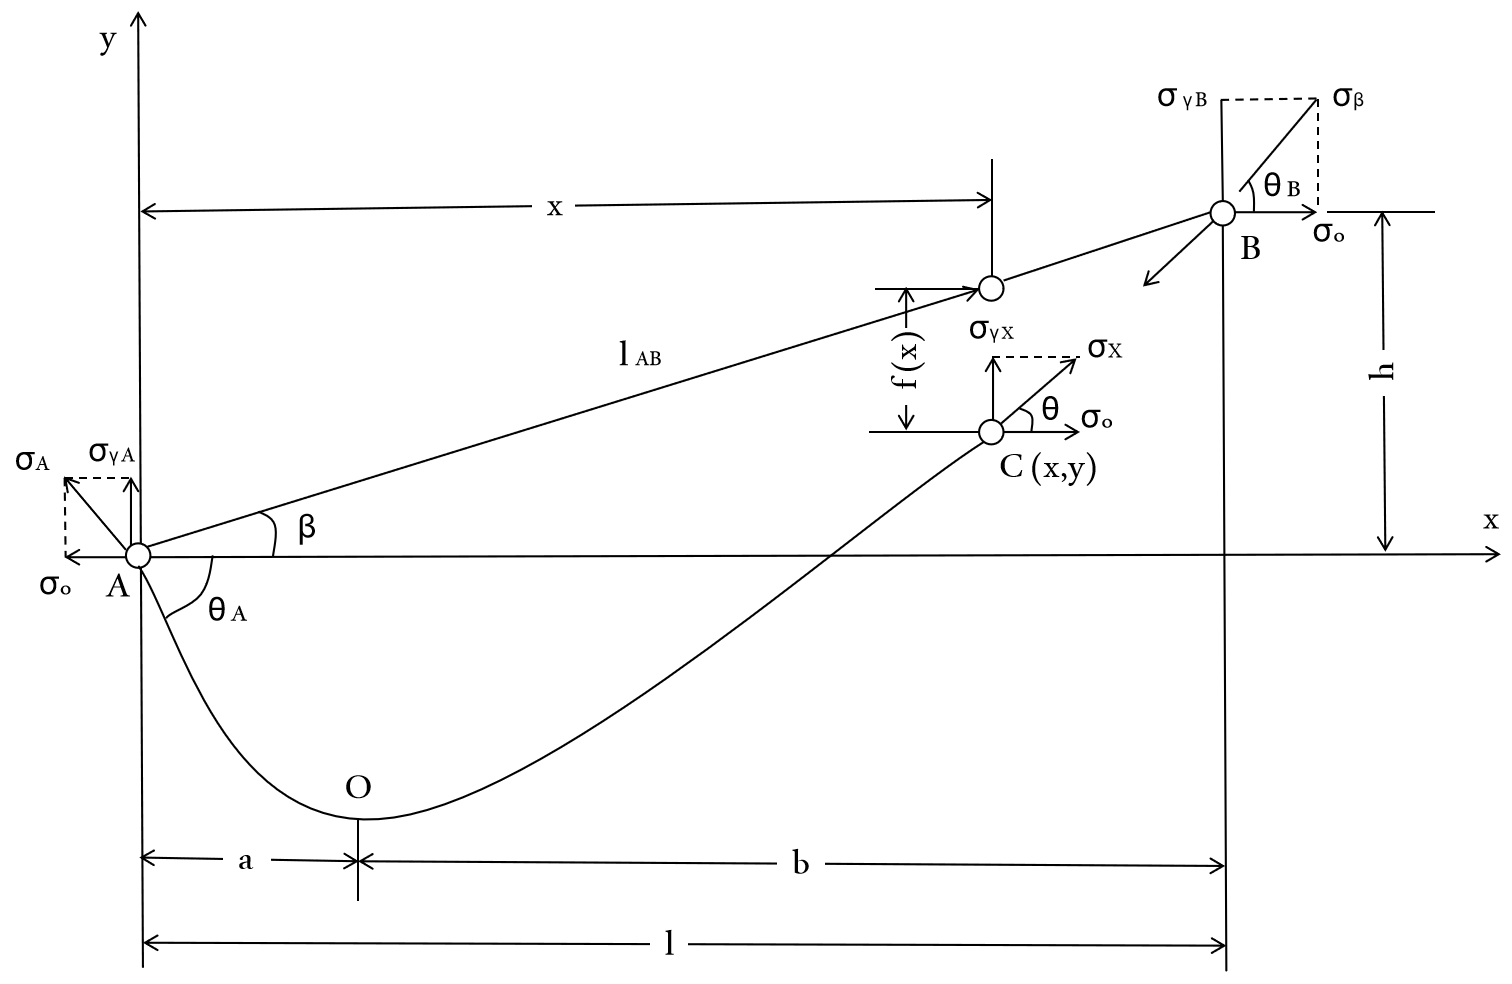
\includegraphics[width=16cm]{figure/悬链线.png}
		\caption*{图八}
	\end{figure}
	\par
	联系我们已获得的数据，OTML获得的角度相当于是$\theta_{A}$与$\theta_{B}$的余角的数据。相当于目前对于一个悬链线系统已知了某一个弧垂角度，可能是$\theta_{A}$也可能是$\theta_{B}$，同时也已知了$tan(\beta)=h/l$。
	\par
	物理学上经常把此时悬链线模型近似为斜抛物线模型[6]进行简化求解，可以得到悬链线最低点处水平应力与弧垂角度的关系。
	\begin{equation}
		tan(\theta_{A})=tan(\beta)-\frac{rl}{2\sigma _{0}\cos\beta  } 
	\end{equation}
	\begin{equation}
		tan(\theta_{B})=tan(\beta)+\frac{rl}{2\sigma _{0}\cos\beta  } 
	\end{equation}
	\par
	其中$A$点是较高点，$B$点是较低点。只要的知某一个点的$\theta$值，结合参数$l,\beta,r$就能求出。参数$r$满足$r=m_{0}/s$。$m_{0}$是每公里的导线质量，s是导线截面积。
	\par
	经过回归拟合发现，$\sigma _{0}$与$t$满足较好的线性关系。
	\begin{figure}[h]
		\small
		\centering
		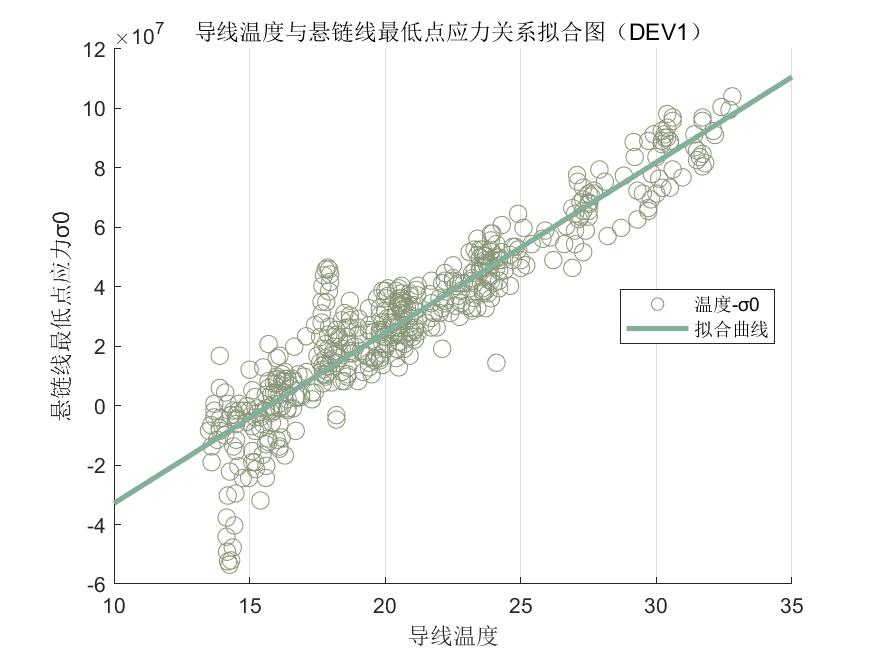
\includegraphics[width=16cm]{figure/应力与导线温度.jpg}
		\caption*{图九}
	\end{figure}
	\par
	得到了公式(14)
	\par
	\begin{equation}
		\sigma _{0}=5.737\times 10^{-6} t_{c}-9.021 \times 10^{-7}
	\end{equation}	
	\par
	其中$5.737\times 10^{-6} $为回归系数$k$。
	\par
	联立公式(12)(14)或(13)(14),就能得到两端点任一弧垂角度与导线温度的关系。
	\par
	\begin{equation}
		t_c=\frac{r l}{2 \cos \beta\left[\tan \left(\frac{\pi}{2}-\theta\right)-\tan \beta\right] k}-\frac{\sigma }{k}
	\end{equation}
	\par
	\subsubsection{模型求解}
	根据公式(1)控制其他变量一定，分别只考虑以$t_{a}$与$t_{c}$为自变量，载流量为因变量得到它们的定量函数关系，如图十所示。
	\begin{figure}[h]
		\small
		\centering
		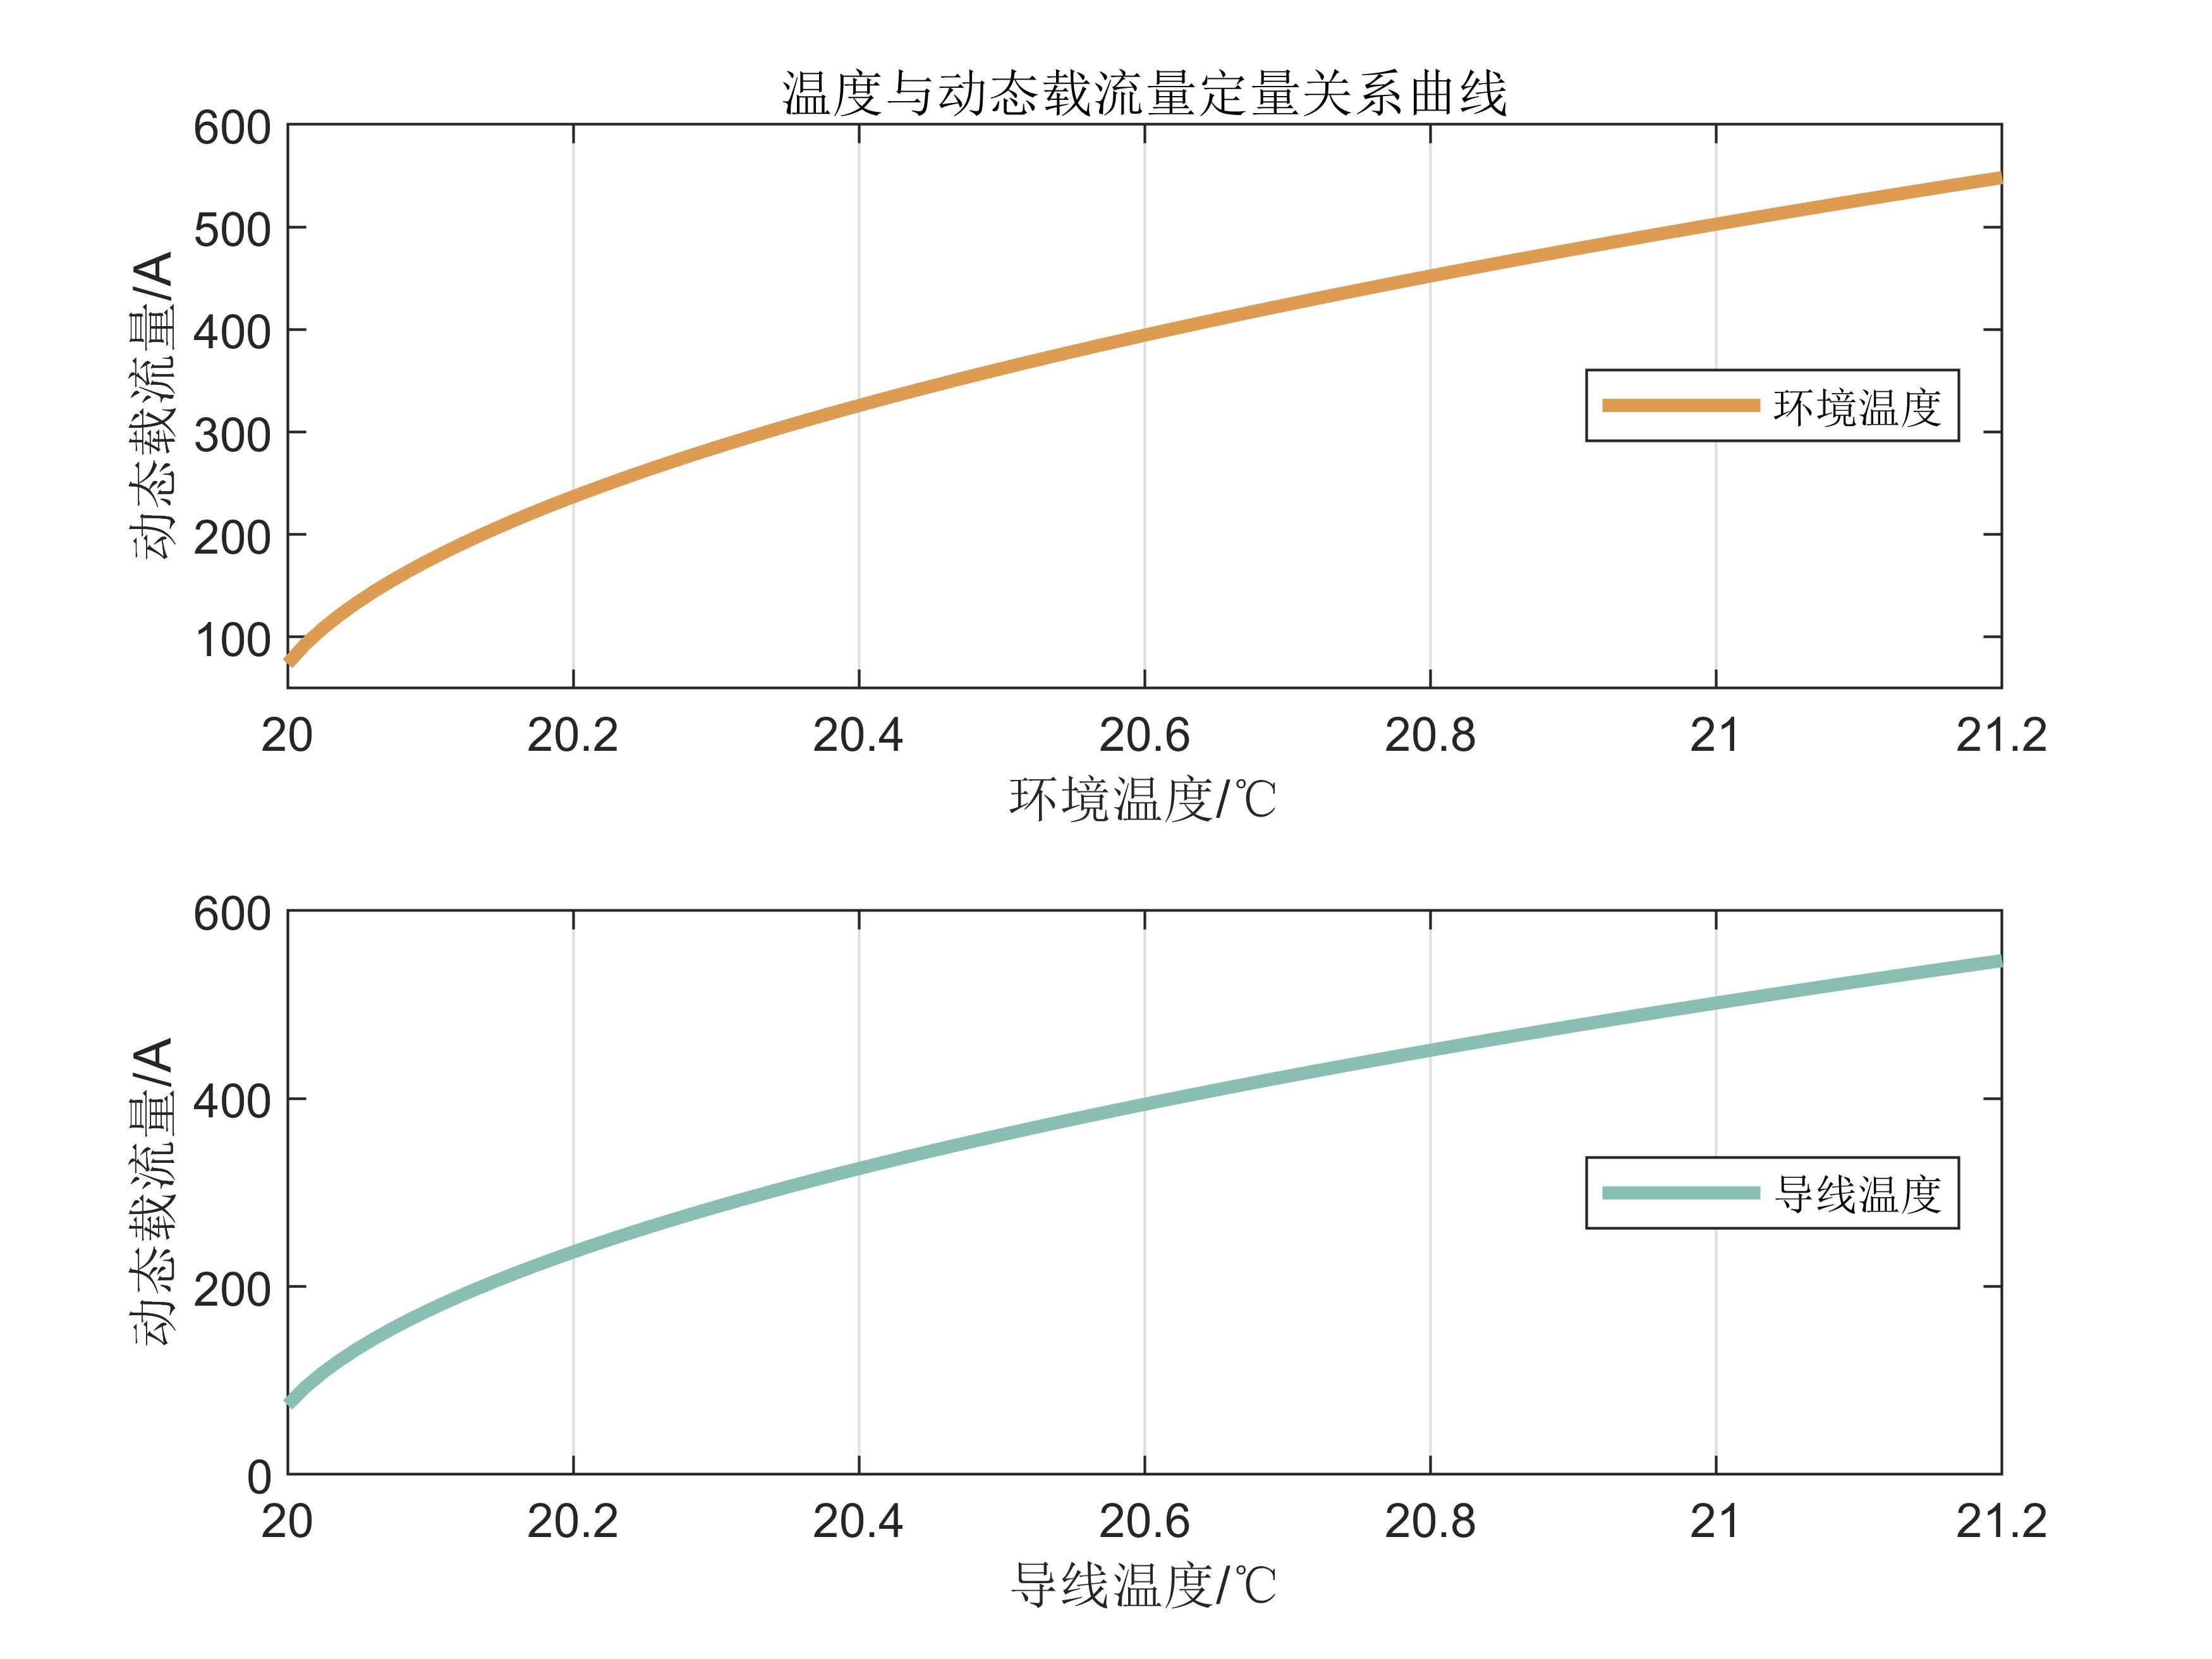
\includegraphics[width=15cm]{figure/温度与载流量.jpg}
		\caption*{图十}
	\end{figure}
	\par
	考虑到两条曲线所代表的变量之间存在一定的相关性，我们在选择数据范围时倾向于一个较小的区间，以确保在这个较小的范围内，这两个变量之间的相互影响可以被视为次要因素，进而可以忽略不计。然而，从更宏观的角度看，这两个变量实际上是共同作用于载流量的，它们共同决定了载流量的变化。这种选择旨在简化分析过程，同时确保结果的准确性。
	\par
	在模型构建的过程中，我们成功地确定了在一般状况下弧垂角度与载流量之间的定量关系。鉴于本题特定的初始条件已明确设定，且我们严格遵循国标选取了相关材料属性，如35/8钢芯铝绞线的电阻等参数，这确保了我们的模型具备高度的针对性和准确性。因此，我们可以精确地描绘出针对本题而言，弧垂角度与载流量之间的具体关系.
	\subsection{问题三的模型建立与求解}
	\subsubsection{模型建立}
	为寻找钢架应力变化与电流变化的关系，我们为此以弧垂角度为桥梁，通过公式推导的方式，分别求出两条道线分别作用与于钢架顶端的作用效果，再将其矢量求和，以其为因变量，对于钢架的四个监测点，两个通道，共八个数据进行多元线性回归，得到其应力与弧垂角度的数学模型；另外，我们通过上一问中弧垂角度与导线温度的定量关系，由于已知导线温度的变化量与质量和比热容的乘机等于功率在时间上的积分，由此算出弧垂角度与电流间关系。
	\subsubsection{问题求解}
	1.弧垂角度与钢架应力关系
	\par
	由第二问建立的模型及公式(12),(13),我们得到了两导线水平最低点的力为分别为：
	$$\sigma _{01} =\frac{rl}{2\cos \beta \left [ \tan \beta -\tan \left ( \pi /2-\theta _{2}  \right )  \right ] } $$
	$$\sigma _{02} =\frac{rl}{2\cos \beta \left [  \tan \left ( \pi /2-\theta _{1}  \right )-\tan \beta  \right ] } $$
	\par
	各角度具体位置如图十一所示。
	\begin{figure}[h]
		\small
		\centering
		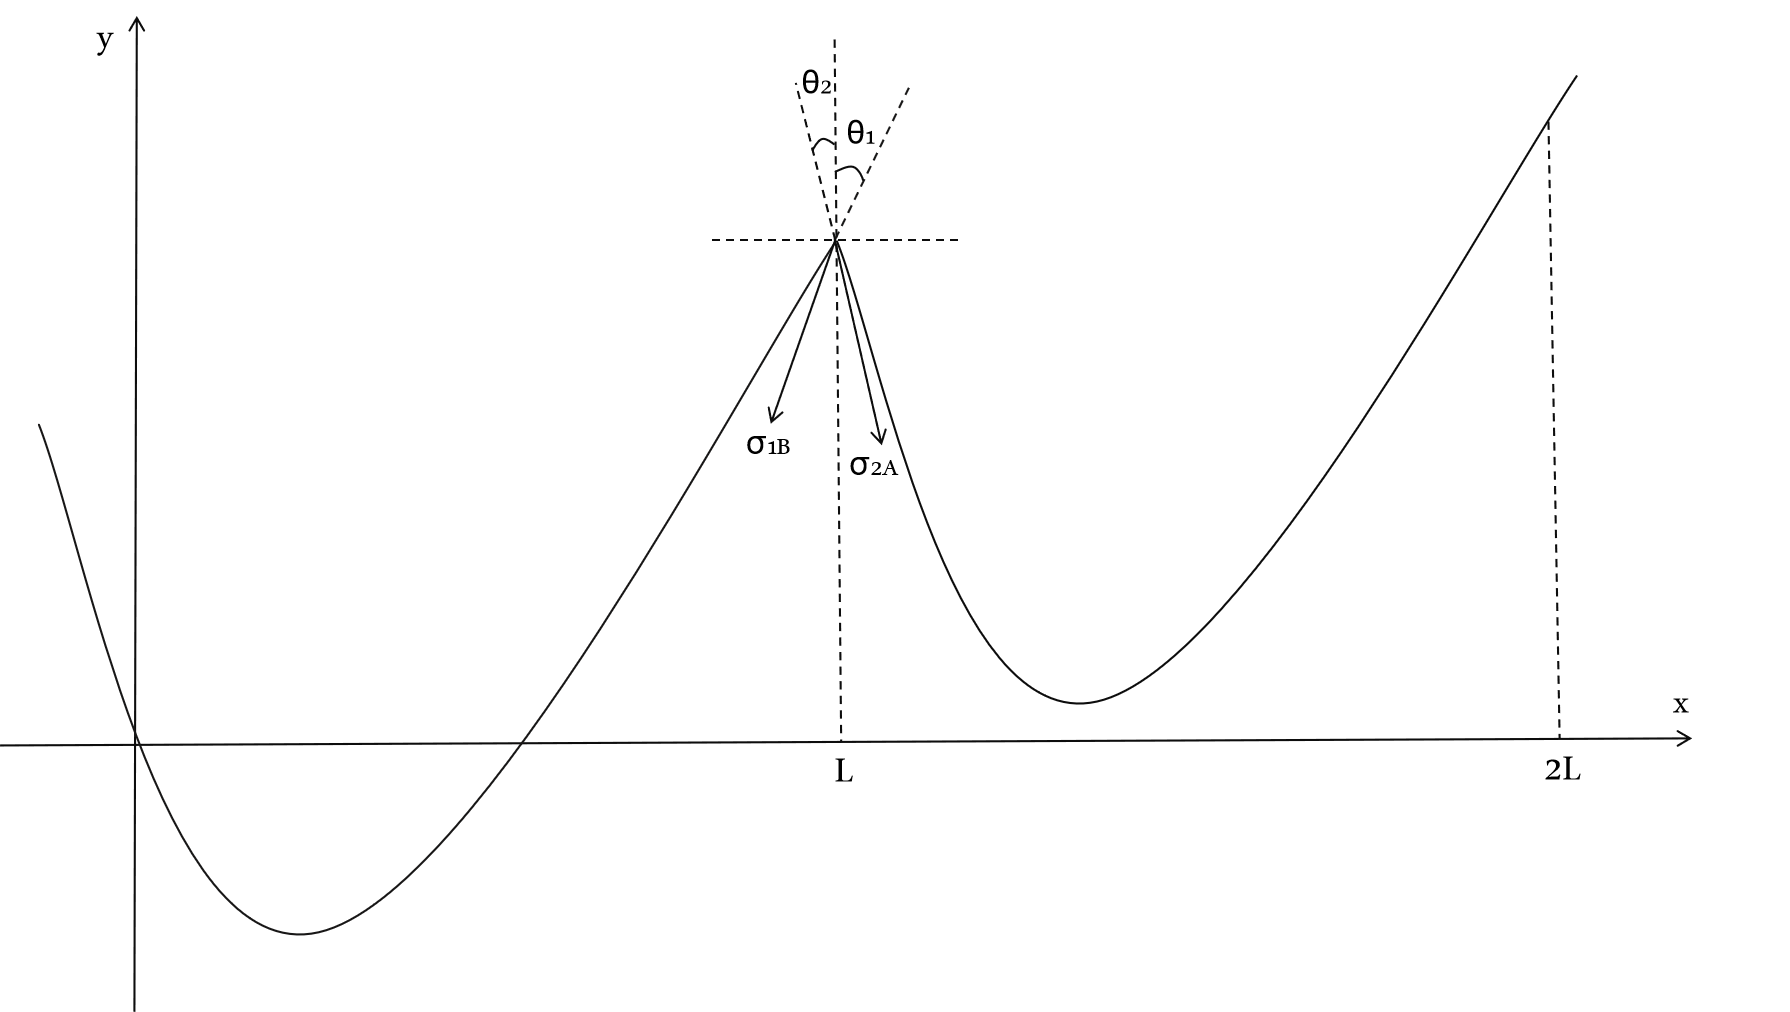
\includegraphics[width=15cm]{figure/题目具象图.png}
		\caption*{图十一}
	\end{figure}
	\par
	通过题目附图已知对于左悬链线有高度差$h_{1}=14m$与档距$l_{1}=160m$，对于右悬链线有高度差$h_{2}=2m$与档距$l_{2}=180m$。
	\par
	为得到两导线对于悬挂点应力，须预先求得各悬链线最大弧垂，由公式(16)斜抛物线方程：
	\begin{equation}
		f_{\mathrm{m}}=\frac{\gamma l^2}{8 \sigma_0 \cos \beta}
	\end{equation}
	\par
	分别可以得到$\sigma_01$,$\sigma_02$。他们是悬链线最低端的水平应力。
	\par
	接下来分别求出左悬链线的右端点悬挂力与右悬链线的左端点悬挂力。得到$\sigma_{1 B}=\frac{\sigma_01}{\cos \beta_1}+r\left(f_{m_1}+\frac{h_1}{2}\right)$,$\sigma_{2 A}=\frac{\sigma_02}{\cos \beta_2}+r\left(f_{m_2}-\frac{h_2}{2}\right)$。
	\par
	
	对其进行矢量合成可以得到合应力:
	$$
	\sigma=\sqrt{\sigma_{2 A^2}+\sigma_{1 B}^2+2 \sigma_{2 A} \sigma_{1 B} \cos \left(\theta_1+\theta_2\right)}
	$$
	对合应力与钢架的八个应力数据进行多元线性回归得到其与钢架应力变化关系$y=\beta_0+\beta_1 x_1+\beta_2 x_2+\cdots+\beta_k x_k+\mu$。其对应的$\beta$值为相应系数，自变量$x$即为钢架的八个应力数据。
	\par
	我们使用matlab的regress函数实现了对其进行了多元线性回归得到系数表如图十二：
	\begin{figure}[h]
		\small
		\centering
		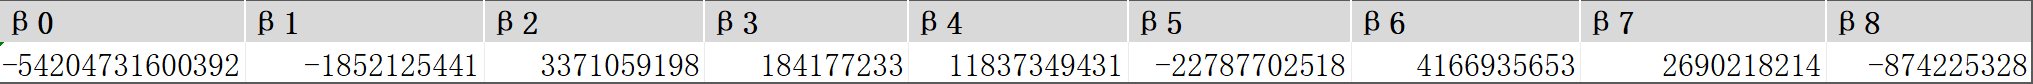
\includegraphics[width=15cm]{figure/8应力回归系数.png}
		\caption*{图十二}
	\end{figure}
	\par
	2.弧垂角度与导线温度的关系
	\par
	通过上一问得到的回归系数$k$得到的弧垂角度与导线温度的关系：$$t_c=\frac{r l}{2 \cos \beta\left[\tan \left(\frac{\pi}{2}-\theta\right)-\tan \beta\right] k}-\frac{\sigma }{k}$$
	\par
	最后得到温度与导线电流关系如下式：
	\begin{equation}
		\begin{aligned}
			& T=\Delta t+T_0=T_0+\frac{Q}{Cm} \\
			= & T_0+\frac{\int I^2 R\left(t_c\right) d t_c}{Cm}
		\end{aligned}
	\end{equation}
	\par
	即得到弧垂角度与导线电流之间的关系,由此以弧垂角度为桥梁的钢架应力变化与电流变化便得以推导。
	\subsection{问题四的求解分析与方案提出}
	\subsubsection{增容需求分析}
	基于第一问建立的动态载流量需求预测模型，我们可以得到基于环境温度与导线温度计算得到的2020年8月15日的电缆所能够承受的最大载流量为$237.1494A$,而经过数据处理预测得到2020年8月15正常用电需求应当为$182.2926A$。但是2020年8月15日用电量大幅提升，有可能超过可承受的最大载流量。
	\subsubsection{增容方式选择}
	在应对2020年8月15日用电量的大幅增加这一暂态短时增容需求时，我们选定了动态增容技术作为解决策略。这种需求指的是在特定条件下，电力系统或电力设备为满足短暂且超出其正常设计容量的需求（如应急需求、高峰负荷等）而进行的临时性增容操作。动态增容技术正是针对这种短时间、突然性的用电需求大幅增加问题的有效解决方案。
	\par
	传统上，在电力电缆的选型和敷设阶段，工程人员为避免电缆在环境温度高时过热从而减少运行寿命，会适当保留负载能力，但这种做法降低了电缆的经济性。相比之下，动态增容技术通过实时监测电缆实际运行的环境与工作情况，能够实时调整电缆的载流量，确保在安全的前提下充分发挥电缆的负载能力。
	\par
	特别是在处理暂态短时增容需求时，动态增容技术相较于传统增容方案（如增大导线截面、增加回路数等）展现出显著优势。它不仅在操作可行性上更高，还降低了人力与物力成本，并提高了电缆的工作效率。因此，针对2020年8月15日用电量的大幅提升问题，我们决定采用动态增容技术作为解决方案。
	\subsubsection{增容方式分析}
	当前，输电线动态增容模型根据其监测对象的不同，可主要划分为两大类别。第一类模型，即气候模型，侧重于对导线所处气象环境如风速、风向、日照、环境温度等的实时监测，从而精准计算导线在特定环境下的载流量。尽管这类模型在业内广泛应用，但由于户外环境中长期使用的风速传感器存在精度局限，其载流量计算结果往往存在一定的误差。
	\par
	第二类动态增容模型则聚焦于部分气象参数与导线状态参数的监测，包括导线温度、弧垂等，涵盖了热路模型、导线温度模型、弧垂模型、张力模型等多种类型。这些模型在载流量计算上的精度较气候模型更高，但它们的实施需要在导线上安装传感器以监测导线状态，这不仅涉及停电操作，还带来了后期维护工作的显著增加，对人力与物力成本提出了较高要求。
	\par
	在动态增容领域，学者们已经取得显著进展。其中，基于规格化建模开发的动态增容暂态计算软件，为稳态负荷与短时负荷的精准计算提供了强有力的支持。此外，提出的双线动态增容策略，在面对双回线路同时需要增容时，提供了灵活的解决方案，可以根据现场需求选择全程启用两回路增容或轮流工作，确保每回线路均匀分担负载。研究指出，对于较短的暂态增容需求，双线增容策略表现出更高的运行效率；而对于长时间增容需求，单线轮流工作则更为理想。
	\par
	根据附件数据，监测点位于中国东北沿海地区，其独特的气候条件，如降水丰富、易受季风影响以及气温变化大等，对动态增容模型的实施提出了挑战。特别是第一类气候模型，其户外传感器的寿命和精度在此类环境下可能受到较大影响。而第二类模型虽然精度高，但安装和维护成本也相对较高。
	\par
	然而，彭向阳等学者提出的基于非接触式等效测量原理的等效散热暂态测量模型[8]，为这一难题提供了解决方案。该模型不仅能够快速准确地评估导线载流量，而且其测量设备独立于导线，安装与维护都相对简便，对监测点所在地区的动态增容实施具有显著的借鉴意义。结合杨洋等学者研究的双线增容策略与动态增容计算软件[7]，我们能够实时获取输电电缆的最大增容量，并根据载流量负荷响应时长，在单线与双线工作模式间做出最优决策。
	
	\section{模型评价}
	\subsection{模型优点}
	1.第一问建立的预测模型将神经网络与时间序列两种预测方法相结合。不但克服了时间序列ARIMA模型由于非线性和结构性变化而难以适应预测区间扩大的缺点，同时也通过引入时间序列的季节性分析功能时神经网络预测结果所呈现的周期性更加明显。两者的结合是应对时间区间相对较长且隐含一定周期性规律的数据序列预测问题的一类新方法。
	\par
	2.第二问建立的回归模型最大的优势是引入相关物理公式，通过公式推导对变量进行转化，将弧垂角度转化为悬链线最低点的应力，进而将其与导线温度进行回归分析。这避免了复杂的悬链线方程而采用工程上的斜抛物线，大大降低了运算的复杂程度，使模型更加简洁，变量间关系的呈现也更加清晰。
	\par
	3.第三问建立的模型，以弧垂角度为桥梁，通过悬链线方程，借助精密的物理推导与数学计算分别构建弧垂角度与导线电流以及弧垂角度与应力之间的关系，使导线电流与应力之间原本模糊的变量关系通过间接而清晰的方式表现出来，抽象关系具体化。同时，链式关系大大拓宽了模型的可应用范围与实用性。
	\par
	4.第四问根据题设条件对电流大幅增加问题进行具体的分类定性，明确了暂态短期载电量的问题性质。针对这一点，本文选择了对该问题的主流解决方式，即采用动态增容模型。同时，在总结各类动态增容模型优缺点的基础上，针对监测点的具体地理情况，本文结合相关资料与研究，提出了具体模型的选择与应用。并结合第一问所得预测模型对最大增容量进行了合理计算。
	\subsection{模型缺陷}
	1.本文神经网络的预测结果并不是绝对理想。对于波动程度过大的数据，基于神经网络只能把握大致的趋势，类似于时间序列季节分析中所获得的季节因子，而难以凸显数据的波动性。
	\par
	2.虽然引入的悬链线方程有助于搭建变量关系，但模型的复杂程度也有所上升。大量复杂的物理公式的引入一定程度上也提高了模型模型的应用难度。
	\section{参考文献}
	\noindent
	[1]戈东方  钟大文  《电力工程电气设计手册1电气一次部分》  水利电力出版社.
	\par\noindent
	[2]戴沅,聂耸,程养春,等.输电线路动态增容载流量计算模型综述[J].广东电力,2012,25(11):51-56.
	\par\noindent  
	[3]孟田华,高清兰,任建光,等.云冈石窟景区晴天太阳辐射模型研究[J].山西大同大学学报(自然科学版),2018,34(01):13-15+52.
	\par\noindent 
	[4]IEC61597(Overheadelectrical conductors－cal culationmethods for strandedbareconductors).
	\par\noindent 
	[5]110kV～750kV架空输电线路设计规范 GB 50545-2010
	\par\noindent 
	[6][精品课程] 不等高悬点架空线的弧垂、线长和应力--架空输电线路设计  三峡大学 输配电线路 2020-07-06 12:07
	\par\noindent 
	[7]杨洋,周韫捷,王媚,李海,陈越超.超高压输电电缆动态增容计算及双线增容策略[J].华东电力,2014,42(09):1774-1779.
	\par\noindent 
	[8]彭向阳,彭瑞东,王锐,郭德明,范亚洲,刘刚.架空输电线路动态增容等效散热暂态测量模型[J].高电压技术,2022,48(10):3975-3986. DOI:10.13336/j.1003-6520.hve.20210783.
	\newpage
	
	\begin{appendices}
		\section*{附录}
		\lstinputlisting[caption={\bf dataclear},]{code/do_clear.m}
		\lstinputlisting[caption={\bf myNeuralNetworkFunction},]{code/myNeuralNetworkFunction.m}
		\lstinputlisting[caption={\bf PredictionRc},]{code/Prediction_of_Rc.m}
		\lstinputlisting[caption={\bf PredictionQc},]{code/Prediction_of_Qc.m}
		\lstinputlisting[caption={\bf PredictionQr},]{code/Prediction_of_Qr.m}
		\lstinputlisting[caption={\bf PredictionQs},]{code/Prediction_of_Qs.m}
		\begin{figure}[htb]
			\small
			\centering
			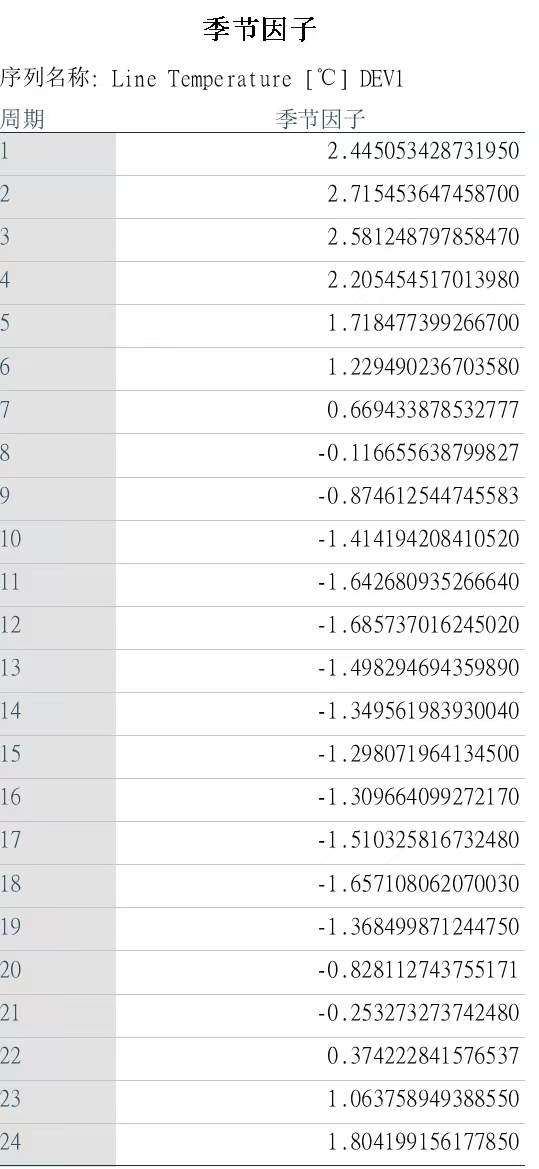
\includegraphics[width=8cm]{figure/季节因子.jpg}
			\caption*{季节因子表}
		\end{figure}
	
	\end{appendices}
\end{document}